\chapter{Diferenciación e Integración numérica\\ Numerical differentiation and integration}
\chaptermark{Difer. e integr. num. \textreferencemark\ NUm. Diff. and Integr. }
\epigraph{You never really understand a person until you consider things from his point of view...until you climb into his skin and walk around in it.}{Harper Lee, To kill a mokingbird}


\begin{paracol}{2}
La diferenciación, y sobre todo la integración son operaciones habituales en cálculo nu\-mérico. En muchos casos obtener la expresión analítica de la derivada o la integral de una función puede ser muy complicado o incluso imposible. Además en ocasiones no disponemos de una expresión analítica para la función que necesitamos integrar o derivar, sino tan solo de un conjunto de valores numéricos de la misma. Este es el caso, por ejemplo, cuando estamos trabajando con datos experimentales. Si solo disponemos de valores numéricos, entonces solo podemos calcular la integral o la derivada numéricamente.

Los sistemas físicos se describen generalmente mediante ecuaciones diferenciales.  La mayoría de las ecuaciones diferenciales no poseen una solución analítica, siendo posible únicamente obtener soluciones numéricas. 

En términos generales la diferenciación nu\-mérica consiste en aproximar el valor que toma la derivada de una función en un punto. De modo análogo, la integración numérica aproxima el valor que toma la integral de una función en un intervalo.

\section{Diferenciación numérica.}
\sectionmark{Diferenciación numérica. \textreferencemark\ Nunerical differentiation.}
Como punto de partida, supondremos que tenemos un conjunto de puntos $\{x_i,y_i\}$,

\switchcolumn


Differentiation and, above all, integration are very common operations in numerical computing. In many cases, obtaining the analytical expression for a function derivative or integral can be very complex or even impossible. Besides, sometimes we have not an analytical expression for the function we need to derivate of integrate, but only a set of numerical values of it. This is the case, for example, when we are worming with experimental data. If we only have numerical values of the function, we can only compute the derivative or integral numerically.

Physical systems are usually describe by differential equations. Most differential equations do not have an analytical solution and thus, we can only obtain numerical solution for them.

In general, numerical differentiation approximates the value taken by the derivative of a function at a specific point. Similarly, numerical integration approximates the value taken by the integral of a function in an interval.

\section{Numerical differentiation.}
We start taking a set of pairs of points $\{x_i,y_i\}$,
\end{paracol}

\begin{table}[h]
\centering
\begin{tabular}{c|cccc}
x&$x_0$&$x_1$&$\cdots$&$x_n$\\
\hline
y&$y_0$&$y_1$&$\cdots$&$y_n$
\end{tabular}
\end{table} 
\begin{paracol}{2}
Que pertenecen a una función $y=f(x)$ que podemos o no conocer analíticamente. El objetivo de la diferenciación numérica es estimar el valor de la derivada $f'(x)$ de la función, en alguno de los puntos $x_i$ en los que el valor de $f(x)$ es conocido. 

En general existen dos formas de aproximar la derivada:

1. Derivando el polinomio de interpolación. De este modo, obtenemos un nuevo polinomio que aproxima la derivada.

\switchcolumn	
Which belong to a function $y = f(x)$ whose analytical expression we may know or may not know. The goal of numerical differentiation is to estimate the value of the function derivative $f'(x)$, in any of the points $x_i$ where the function value $f(x)$ is known.

We can distinguish two different method to approximate the derivative:

1. WE can derivate the polynomial that interpolates the point. So, we get a new polynomial that approximate the derivative.  
\end{paracol}
\begin{equation*}
f(x)\approx P_n(x) \Rightarrow f'(x) \approx P'_n(x)
\end{equation*}
\begin{paracol}{2}
2. Estimando la derivada como una fórmula de diferencias finitas obtenida a partir de la aproximación del polinomio de Taylor. 

Si partimos de la definición de derivada,

\switchcolumn
2. Estimating the derivativa using a finite differences quotient obtained from the Taylor polinomial expansion.

If we start from the definition of derivative,
\end{paracol} 
\begin{equation*}
f'(x_0)=\lim_{h\rightarrow 0}\frac{f(x_0+h)-f(x_0)}{h} \approx \frac{f(x_0+h)-f(x_0)}{h} 
\end{equation*}
\begin{paracol}{2}
Podemos asociar esta aproximación con el polinomio de Taylor de primer orden de la función $f(x)$,
\switchcolumn
We can associate this approach with the first-degree Taylor polynomial expansion of functions $f(x)$
\end{paracol}
\begin{equation*}
f(x)\approx f(x_0)+f'(x_0)\cdot(x-x_0) \Rightarrow f'(x_0)\approx \frac{f(x)-f(x_0)}{x-x_0}
\end{equation*}
\begin{paracol}{2}
Si hacemos $x-x_0=h$, ambas expresiones coinciden.
 
En general, los algoritmos de diferenciación numérica son inestables. Los errores iniciales que puedan contener los datos debido a factores experimentales o al redondeo del ordenador, aumentan en el proceso de diferenciación. Por eso no se pueden calcular derivadas de orden alto y, los resultados obtenidos de la diferenciación numérica deben tomarse siempre extremando la precaución.

\subsection{Diferenciación numérica basada en el polinomio de interpolación.}\index{Diferenciación! polinomio interpolador}

El método consiste en derivar el polinomio $P_n(x)$ de interpolación obtenido por alguno de los métodos estudiados en el capítulo \ref{interpolacion} y evaluar el polinomio derivada $P'_n(x)$ en el punto deseado.

Un ejemplo particularmente sencillo, para la expresión del polinomio derivada se obtiene  en el caso de datos equidistantes interpolados mediante el polinomio de Newton-Gregory,
\switchcolumn	
If we take $x-x_0 = h$ both expressions meet.

In general, the numerical differentiation algorithms are unstable. Initial data errors due to experimental factors or computer rounding off increase with the differentiation process. For this reason, it is not possible to compute high-order derivatives, and the results achieved from numerical differentiation must always be considered extremely carefully.

\subsection{Numerical differentiation\\ base on the interpolation polynomial.}\index[eng]{differentiation! interpolation polynomial}

The method involves deriving the polynomial $P_n(x)$ using any of the methods described in chapter \ref{interpolacion} and then evaluating the derivative polynomial $P_n'(x)$ at the desired point.

WE can obtain a specially simple expression for the derivative polynomial, in the case o equispaced points interpolated by the newton-Gregory polynomial, 
\end{paracol}
\begin{equation*}
p_n(x)=y_0+\frac{x-x_0}{h}\Delta y_0+\frac{(x-x_1)\cdot (x-x_0)}{2\cdot h^2}\Delta^2 y_0+\cdots +\frac{(x-x_{n-1}) \cdots (x-x_1)\cdot (x-x_0)}{n! \cdot h^n}\Delta^n y_0
\end{equation*}
\begin{paracol}{2}
Si lo derivamos, obtenemos un nuevo polinomio,
\switchcolumn
And after deriving, we obtain a new polynomial,
\end{paracol}
\begin{align*}
p'_n(x)&=\frac{\Delta y_0}{h}+\frac{\Delta^2 y_0}{2\cdot h^2}\left[(x-x_1)+(x-x_0) \right] +\\
&+\frac{\Delta^3 y_0}{3! \cdot h^3}\left[(x-x_1)(x-x_2)+(x-x_0)(x-x_1)+(x-x_0)(x-x_2)\right]+\cdots +\\
&+\frac{\Delta^n y_0}{n! \cdot h^n}\sum_{k=0}^{n-1}\frac{(x-x_0)(x-x_1)\cdots (x-x_{n-1})}{x-x_k}
\end{align*}
\begin{paracol}{2}
Este polinomio es especialmente simple de evaluar en el punto $x_0$,
\switchcolumn
To evaluate this polynomial at point $x_0$ is particularly easy,
\end{paracol}
\begin{align*}
p'_n(x_0)&=\frac{\Delta y_0}{h}+\frac{\Delta^2 y_0}{2\cdot h^2}\overbrace{(x_0-x_1)}^{-h}+\cdots +
\frac{\Delta^n y_0}{n! \cdot h^n}[\overbrace{(x_0-x_1)}^{-h}\overbrace{(x_0-x_2)}^{-2h}\cdots \overbrace{(x_0-x_{n-1})}^{-(n-1)h}]\\
p'_n(x_0)&=\frac{1}{h}\left(\Delta y_0-\frac{\Delta^2 y_0}{2}+\frac{\Delta^3 y_0}{3}+\cdots +
\frac{\Delta^n y_0}{n}(-1)^{n-1}\right)
\end{align*}
\begin{paracol}{2}
Es interesante remarcar como en la expresión anterior, el valor de la derivada se va haciendo más preciso a medida que vamos añadiendo diferencias de orden superior. Si solo conociéramos dos datos, $(x_0, y_0)$ y $(x_1, y_1)$, solo podríamos calcular la diferencia dividida de primer orden. En este caso nuestro cálculo aproximado de la derivada de $x_0$ sería,
\switchcolumn
It is worth notice that the previous expression represent de derivative with increasing precision as we add new higher-order differences. If we would only know two data, $(x_0,y_0)$ y $(x_1,y_1)$, we could only calculate the first-order divided difference. In which case, our approximate derivative computation at $x_0$ would be,  

\end{paracol}
\begin{equation*}
p'_1(x_0)=\frac{1}{h}\Delta y_0
\end{equation*}
\begin{paracol}{2}
Si conocemos tres datos, podríamos calcular $\Delta^2y_0$ y añadir un segundo término a nuestra estima de la derivada,
\switchcolumn
If we have three data, we could compute $\Delta^2y_0$ and add second term to our derivative estimation.
\end{paracol}
\begin{equation*}
p'_2(x_0)=\frac{1}{h}\left(\Delta y_0-\frac{\Delta^2 y_0}{2}\right)
\end{equation*}
\begin{paracol}{2}
y así sucesivamente, mejorando cada vez más la precisión.

Veamos como ejemplo el cálculo la derivada en el punto $x_0=0.0$ a partir de la siguiente tabla de datos,
\switchcolumn
And so on, precision is increasingly improving.

Let see the computing of the derivative at point $x_0 =0.0$ using the following data table,
\end{paracol}
\begin{table}[h]
\centering
\begin{tabular}{cccccc}
$x_i$&$y_i$&$\Delta y_i$&$\Delta^2 y_i$&$\Delta^3 y_i$ & $\Delta^4 y_i$\\
\hline
$0.0$& $0.000$& $0.203$ &$0.017$ &$0.024$ &$0.020$\\
$0.2$ &$0.203$ &$0.220$ &$0.041$ &$0.044$\\
$0.4$ &$0.423$ &$0.261$ &$0.085$\\
$0.6$ &$0.684$ &$0.346$\\
$0.8$ &$1.030$\\
\end{tabular}
\end{table} 

\begin{paracol}{2}
1. Empleando los dos primeros puntos,
\switchcolumn
1. Using the two first points,
\end{paracol}
\begin{equation*}
y'(0,0)=p_1^1(0.0)=\frac{1}{0.2}\cdot 0.203= 1.015
\end{equation*}
\begin{paracol}{2}
2. Empleando los tres primeros puntos,
\switchcolumn
2. Using the three first points,
\end{paracol}
\begin{equation*}
y'(0,0)=p_2^1(0.0)=\frac{1}{0.2}\left( 0.203-\frac{0.017}{2}\right)= 0.9725
\end{equation*}
\begin{paracol}{2}
3. Empleando los cuatro primeros puntos,
\switchcolumn
3. Using the four first points,
\end{paracol}
\begin{equation*}
y'(0,0)=p_3^1(0.0)=\frac{1}{0.2}\left( 0.203-\frac{0.017}{2}+\frac{0.024}{3}\right)= 1.0125
\end{equation*}
\begin{paracol}{2}
4. Empleando los cinco puntos disponibles,
\switchcolumn
4. Using the four available points,
\end{paracol}
\begin{equation*}
y'(0,0)=p_4^1(0.0)=\frac{1}{0.2}\left( 0.203-\frac{0.017}{2}+\frac{0.024}{3}-\frac{0.020}{4}\right)= 0.9875
\end{equation*}

\begin{paracol}{2}
\subsection{Diferenciación numérica basada\\ en diferencias finitas}
\index{Diferenciación! diferencias finitas}
Como se explicó en la introducción, la idea es emplear el desarrollo de Taylor para aproximar la derivada de una función en punto. Si empezamos con el ejemplo más sencillo, podemos aproximar la derivada suprimiendo de su definición el \emph{paso al límite}\index{Diferenciación!Diferencia adelantada de dos puntos},

\switchcolumn
\subsection{Numerical differentiation base\\ on finite differences}
\index[eng]{Differentiation! finite differences}
As we explained in the introduction to the chapter, the idea is to take the Taylor's expansion to approximate a function derivative at a specific point. If we start with the simplest case, we can approximate the derivative suppressing the \emph{limit computation} in its definition\index[eng]{Diferentiation! Two point forward diference}
\end{paracol}
\begin{equation*}
f'(x_k)=\lim_{h\rightarrow 0}\frac{f(x_k+h)-f(x_k)}{h} \approx \frac{f(x_k+h)-f(x_k)}{h} 
\end{equation*}
\begin{paracol}{2}
La expresión obtenida, se conoce con el nombre de formula de diferenciación adelantada de dos puntos. El error cometido debido a la elección de un valor de $h$ finito, se conoce con el nombre de error de truncamiento\index{Error de Truncamiento}. Es evidente que desde un punto de vista puramente matemático, la aproximación es mejor cuanto menor es $h$. Sin embargo, desde un punto de vista numérico esto no es así. A medida que hacemos más pequeño el valor de $h$, aumenta el error de redondeo debido a la aritmética finita del computador\index{Error de redondeo}. Por tanto, el error cometido es la suma de ambos errores,
\switchcolumn
The expression we have achieved is know as two-point forward difference formula. The error we make due to the finite value we chose for $h$ is called as truncation error. It is clear that from a purely mathematical point of view, the approximation is better the smaller $h$ is. However, this is not true from a numerical point of view. As we make smaller the value of $h$, the rounding-off error increases due to the computer finite arithmetic. Then we have to take into account the sum of both errors,   
\end{paracol}
\begin{equation*}
f'(x)=\frac{f(x+h)-f(x)}{h}+\underbrace{\overbrace{C\cdot h}^{\mathrm{ truncating}}}_{\mathrm{truncamiento}}+\underbrace{\overbrace{D\cdot \frac{1}{h}}^{redondeo}}_{\mathtt{rounding}}, \ C>>D 
\end{equation*}
\begin{paracol}{2}
El valor óptimo de $h$ es aquel que hace mínima la suma del error de redondeo y el error de truncamiento. La figura \ref{fig:errores} muestra de modo esquemático como domina un error u otro según hacemos crecer o decrecer el valor de $h$ en torno a su valor óptimo.
\switchcolumn

The optimal value for $h$ is that what minimised the rounding-off error plus the truncating error sum. figure \ref{fig:errores} shows schematically  how truncating or rounding-off error dominates as we do grow or decrease the value of $h$ around its optimal value.
\end{paracol}
\begin{figure}[h]
\centering
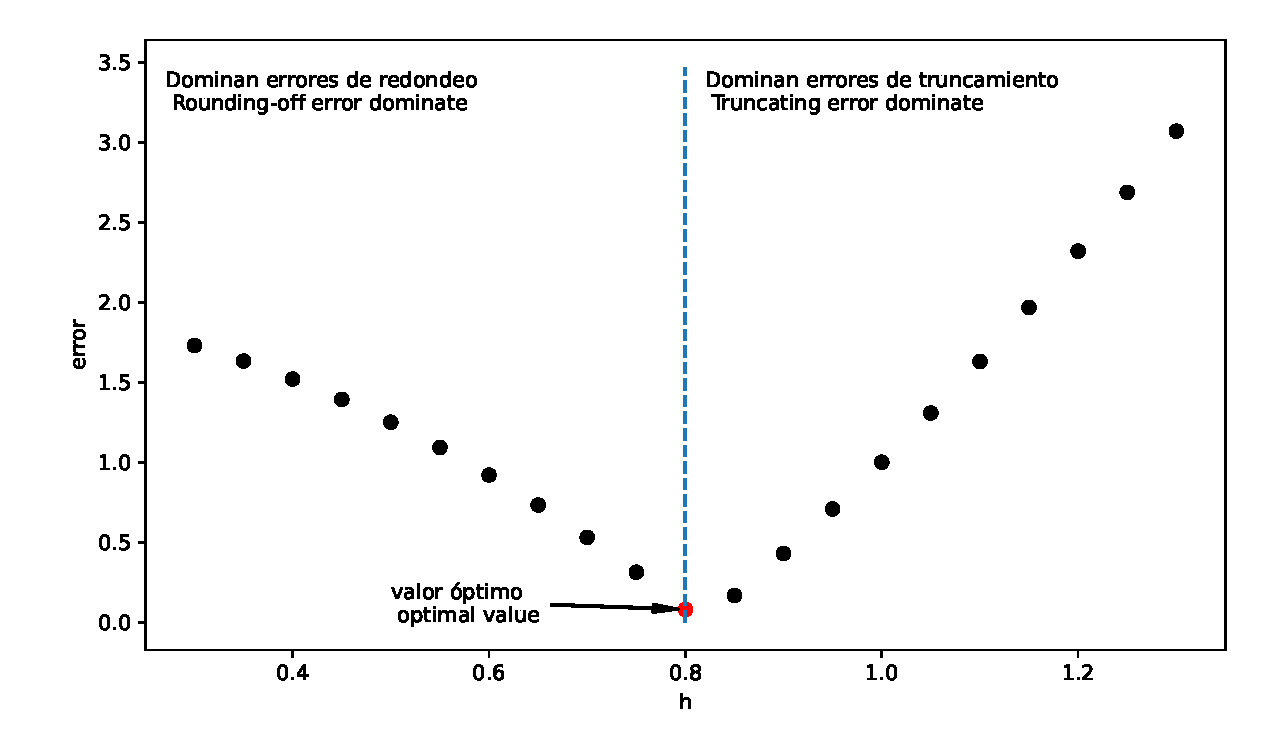
\includegraphics[width=12cm]{errores.eps}
\bicaption{Variación del error cometido al aproximar la derivada de una función empleando una fórmula de diferenciación de dos puntos.}{Function derivative approximation error, using a a two-points differentiation formula. Dependency on the difference $h$ value} 
\label{fig:errores}
\end{figure}
\begin{paracol}{2}
Como vimos en la introducción a esta sección, partiendo de el desarrollo de Taylor de una función es posible obtener fórmulas de diferenciación numérica y poder estimar el error cometido. Así por ejemplo, a  partir del polinomio de Taylor de primer orden,
\switchcolumn
A we sow in the introducction to the present section, departing from a function Taylor's expansion it is possible to arrive to different numerical differentiation formulae and estimate the error made. So, for instance, departing from the fist order Taylor's polynomial,
\end{paracol}
\begin{equation*}
f(x+h)=f(x)+hf'(x)+\frac{h^2}{2}f''(z) \Rightarrow f'(x)=\frac{f(x+h)-f(x)}{h}-\frac{h}{2}f''(z), \ x<z<x+h
\end{equation*}
\begin{paracol}{2}
El error que se comete debido a la aproximación, es proporcional al tamaño del intervalo empleado $h$ La constante de proporcionalidad depende de la derivada segunda de la función, $f''(z)$ en algún punto indeterminado $z\in (x,x+h)$. Para indicar esta relación lineal entre el error cometido y el valor de $h$, se dice que el error es del \emph{orden} de $h$ y se representa como $O(h)$.
\switchcolumn
The error we make is proportional to the interval $h$ that we use. The constant of proportionality depends on the second derivative of the function, $f''(z)$, at an undetermined point $z \in (x, x+h)$. We express this error as having a linear dependency on the value of $h$, stating that the error is of order $h$, and we represent it as $O(h)$.
\end{paracol}
\begin{equation*}
f'(x)=\frac{f(x+h)-f(x)}{h}+O(h)
\end{equation*}

\begin{figure}[h]
\centering
\begin{subfigure}{0.45\textwidth}
	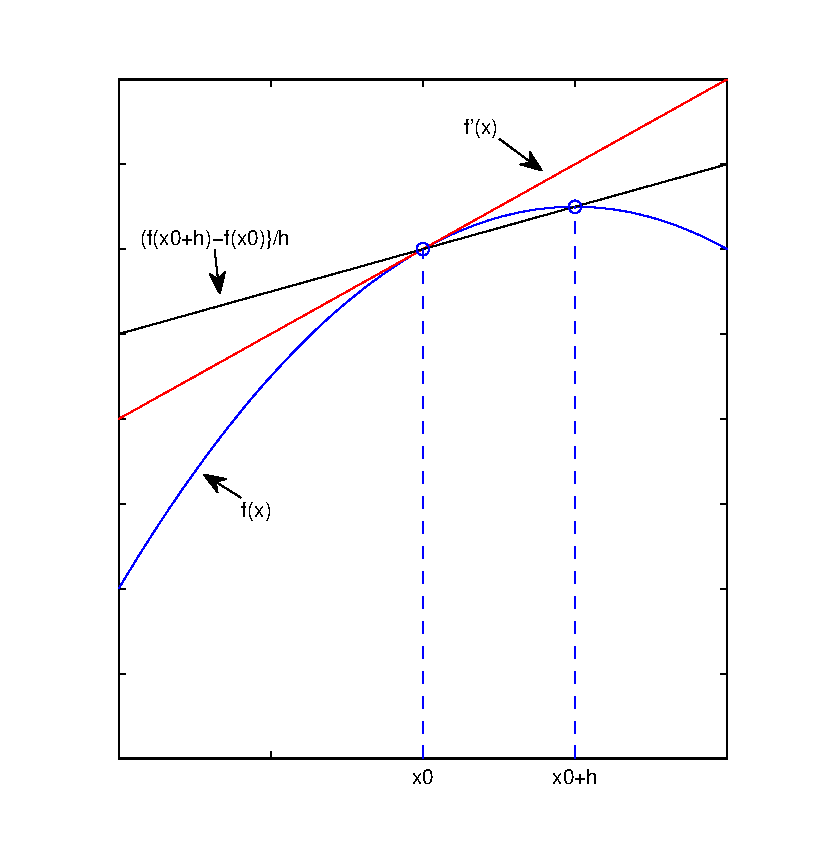
\includegraphics[width=7cm]{diffin1.eps}
	\bicaption{Diferencia de dos puntos adelantada}{Two points forward difference} \label{fig:diffin1}
\end{subfigure} 
\begin{subfigure}{0.45\textwidth}
	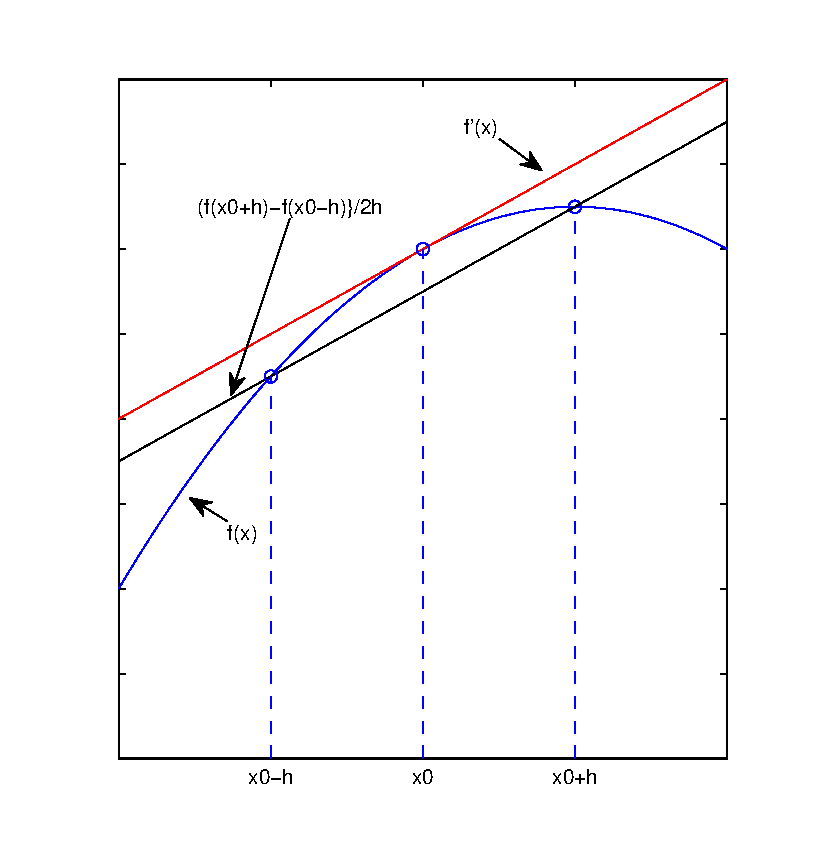
\includegraphics[width=7cm]{diffin2.eps}
	\bicaption{Diferencia de dos puntos centrada}{Two point central difference} \label{fig:diffin2}
\end{subfigure}
\bicaption{Comparación entre las aproximaciones a la derivada de una función obtenidas mediante las diferencias de dos puntos adelantada y centrada.}{Comparison between the approximations achieved for a function derivative using two point forward difference and two point central difference.}
\label{fig:diffin}
\end{figure}
\begin{paracol}{2}
Podemos mejorar la aproximación, calculando el valor de polinomio de Taylor de tercer orden para dos puntos equidistantes situados a la izquierda y la derecha del punto x, restando dichas expresiones y despejando la derivada primera del resultado,

\switchcolumn

To enhance the accuracy, we can calculate the value of the third-order Taylor polynomials at two equally spaced points to the left and right of the point x. Then we find the difference between these values and solve for the first derivative.
\end{paracol}
\begin{equation*}
\left. \begin{aligned}
f(x+h)=f(x)+hf'(x)+\frac{h^2}{2}f''(x)+\frac{h^3}{3!}f'''(z)\\
f(x-h)=f(x)-hf'(x)+\frac{h^2}{2}f''(x)-\frac{h^3}{3!}f'''(z)
\end{aligned} \right\rbrace \Rightarrow f'(x)=\frac{f(x+h)-f(x-h)}{2h}-\frac{h^2}{6}f'''(z) 
\end{equation*}
\begin{paracol}{2}
En esta caso, el error es proporcional al cuadrado de $h$, por tanto,
\switchcolumn
In this case, we get an error proportional to $h$ square, thus,
\end{paracol}
\begin{equation*}
f'(x_0)=\frac{f(x_1)-f(x_{-1})}
{2h}+O(h^2)
\end{equation*}
\begin{paracol}{2}
Donde hemos hecho $x\equiv x_0$, $x+h\equiv x_1$ y $x-h\equiv x_{-1}$. Esta aproximación recibe el nombre de diferencia de dos puntos centrada.\index{Diferenciación! Diferencia de dos puntos centrada} La figura \ref{fig:diffin1} muestra una comparación entre la derivada real de una función y su aproximación mediante una diferencia adelantada de dos puntos. La figura \ref{fig:diffin2} muestra la misma comparación empleando esta vez la aproximación de dos punto centrada. En este ejemplo es fácil ver como la aproximación centrada da un mejor resultado. No hay que olvidar que  la bondad del resultado, para un valor de $h$ dado, depende también del valor de las derivadas de orden superior de la función, por lo que no es posible asegurar que el resultado de la diferencia centrada sea siempre mejor.

Empleando el desarrollo de Taylor y tres puntos podemos aproximar la derivada por la diferencia de tres puntos adelantada,
\switchcolumn
Where we have taken $x\equiv x_0$, $x+h\equiv x_1$ y $x-h\equiv x_{-1}$. This approximation is called two point central difference.\index{Diferentiation! Two point central difference} Figure \ref{fig:diffin1} shows a comparison between an actual function derivative and its approximation using a two point forward difference formula. Figure \ref{fig:diffin2} Compares, for the same function, the actual derivative with a two points central difference approximation. In this example, we can see how the central approximation yields better results. However, the accuracy of a result also depends on the higher-order derivative values of the function.  Therefore, it is not possible to claim that the central difference will always result in better outcomes.

 With three points and the Tylor's expansion we can approximate the derivative using a three points forward difference formula,   
\end{paracol}
\begin{align*}
\left. \begin{aligned}
4\cdot\left(f(x_1)=f(x_0)+hf'(x_0)+\frac{h^2}{2}f''(x_0)+\frac{h^3}{3!}f'''(z)\right)\\
f(x_2)=f(x_0)+2hf'(x_0)+2{h^2}{2}f''(x_0)+\frac{4h^3}{3}f'''(z)
\end{aligned} \right\rbrace \Rightarrow \\
\Rightarrow f'(x_0)=\frac{-f(x_2)+4f(x_1)-3f(x_0)}{2h}-\frac{h^2}{3}f'''(z) 
\end{align*} 
\begin{paracol}{2}
En este caso e error es también de  orden $h^2$ pero vale el doble que para la diferencia de dos puntos centrada.

A partir del desarrollo de Taylor y mediante el uso del número de puntos adecuado, es posible obtener aproximaciones a la derivada primera y a las sucesivas derivadas de una función, procediendo de modo análogo a como acaba de mostrarse para el caso de las diferencias de dos y tres puntos. La tabla \ref{tabdiff} muestra algunas de las fórmulas de derivación mediante diferencias finitas más empleadas. Para simplificar la notación, en todos los casos se ha tomado $y_i=f(x_i), \ y_i^{(j)}=f^{(j)}(x_i)$.

\switchcolumn
In this case the also get a order $h^2$ error but its two times the value achieved for the two point central difference.

From Taylor's expansion and using the appropriated number of points, it si possible to compute approximation for the first and successive derivatives of a function. The procedure is similar to the one we employed in the two and tree points differences. Table \ref{tabdiff} shows some derivative approximations using the most common finite differences formulae. To simplify notation, in every case we have taken $y_i=f(x_i), \ y_i^{(j)}=f^{(j)}(x_i)$. 

\end{paracol}
\begin{table}[h]
\centering
\begin{tabular}{|c|c|}
\hline
Fórmulas primera derivada & Fórmulas segunda derivada\\
First derivative formulae & Second derivative formulae\\
\hline
\ & \\
$y'_0=\frac{y_1-y_0}{h}+O(h)$ & $y''_0=\frac{y_2-2y_1+y_0}{h^2}+O(h)$\\
\ & \\
$y'_0=\frac{y_1-y_{-1}}{2h}+O(h^2)$ &$y''_0=\frac{y_1-2y_0+y_{-1}}{h^2}$\\
\ & \\
$y'_0=\frac{-y_2+4y_1-3y_0}{2h}+O(h^2)$ &$y''_0=\frac{-y_3+y_2-5y_1+2y_0}{h^2}+O(h^2)$\\
\ & \\
$y'_0=\frac{-y_2+8y_1-8y_{-1}+y_{-2}}{12h}+O(h^4)$ &$y''_0=\frac{-y_2+16y_1-30y_0+16y_{-1}-y_{-2}}{12h^2}+O(h^4)$\\
\ & \\
\hline
Fórmulas tercera derivada & Fórmulas cuarta derivada\\
Third derivative formulae & Fourth derivative formulae\\
\hline
\ & \\
$y'''_0=\frac{y_3-3y_2+3y_1-y_0}{h^3}+O(h)$ &$y^{iv}_0=\frac{y_4-4y_3+6y_2-4y_1+y_0}{h^4}+O(h)$\\
\ & \\
$y'''_0=\frac{y_2-2y_1+2yx_{-1}-y_{-2}}{2h^3}+O(h^2)$ &$y^{iv}_0=\frac{y_2-4y_1+6y_0-4y_{-1}+y_{-2}}{h^4}+O(h^2)$\\
\ &  \\
\hline
\end{tabular}
\bicaption{Fórmulas de derivación basadas en diferencias finitas}{Derivative formulae based on finite differences}
\label{tabdiff}
\end{table}

\begin{paracol}{2}
\section{Integración numérica.}\label{sec:inum}
\sectionmark{Integración numérica. \textreferencemark\ Numerical Integration.}

Dada una función arbitraria $f(x)$ es en muchos casos posible obtener de modo analítico su primitiva $F(x)$ de modo que $f(x)=F'(x)$. En estos casos, la integral definida de $f(x)$ en un intervalo $[a,b]$ puede obtenerse directamente a partir de su primitiva,

\switchcolumn
\section{Numerical Integration.}
Given an arbitrary function $f(x)$ it is in many cases possible to obtain analitically is primitive $F(x)$ such that, $f(x)=F'(x)$. In these cases, the function $f(x)$ definite integral in an interval $[a,b]$ can be obtained from its primitive.

\end{paracol}
\begin{equation*}
I(f)=\int_a^bf(x)dx=F(x)\vert_a^b=F(b)-F(a)
\end{equation*}
\begin{paracol}{2}
Hay sin embargo muchos casos en los cuales se desconoce la función $F(x)$ y otros en los que ni siquiera se conoce la expresión de la función $f(x)$, como por ejemplo, cuando solo se dispone de una tabla de valores $\{ x_i,y_i=f(x_i) \}$ para representar la función. En estos casos se puede aproximar la integral definida de la función $f(x)$ en un intervalo $[a,b]$, a partir de los puntos disponibles, mediante lo que se conoce con el nombre de una fórmula de cuadratura,

\switchcolumn
There are many cases for which we do not know function $F(x)$, and there are others where we do not even know the function $f(x)$ as, for example, when we only have a data table $\{x_i,y_i = f(x_i)\}$ that represents the function. In these cases, it is possible to approximate the de definite integral of a function $f(x)$ in an interval $[a,b]$ using available points and methods known as quadrature formulae.
\end{paracol}
\begin{equation*}
I(f)=\int_a^bf(x)dx \approx \sum_{i=0}^nA_if(x_i)
\end{equation*}
\begin{paracol}{2}
Una técnica habitual de obtener los coeficientes $A_i$, es hacerlo de modo implícito a partir de la integración  de los polinomios de interpolación,
\switchcolumn
A common  technique to obtain $A_i$ coefficients is to use an implicit method by interpolating polynomial integration,
\end{paracol}
 \begin{equation*}
I(f)=\int_a^bf(x)dx \approx \int_a^bP_n(x)dx
\end{equation*}
\begin{paracol}{2}
Para ello, se identifican los extremos del intervalo de integración con el primer y el último de los datos disponibles, $[a,b]\equiv [x_0,x_n]$.

Así por ejemplo, a partir de los polinomios de Lagrange, definidos en la sección \ref{sec:lagranje},
\switchcolumn
To do this, we first takes the ends of the interval as the first and last data available, $[a,b]\equiv [x_0,x_n]$.

So, for example, we using Lagrange's polynomials defined in section \ref{sec:lagranje},
\end{paracol}
\begin{equation*}
p(x)=\sum_{j=0}^n l_j(x)\cdot y_j
\end{equation*}
\begin{paracol}{2}
Podemos obtener los coeficientes $A_i$ como,
\switchcolumn	
We can compute the $A_i$ coefficientes as,
\end{paracol}
\begin{equation*}
I(f)=\int_a^bf(x)dx \approx \int_a^bP_n(x)dx=\int_{x_0}^{x_n}\left( \sum_{j=0}^n l_j(x)\cdot y_j \right) dx \Rightarrow A_j=\int_{x_0}^{x_n}l_j(x)dx
\end{equation*}
\begin{paracol}{2}
La familia de métodos de integración, conocidas como fórmulas de Newton-Cotes, puede obtenerse a partir del polinomio de interpolación de Newton-Gregory descrito en la sección \ref{sec:newgre}\index{Integración! Formulas de Newton-Cotes}. Supongamos que tenemos la función a integrar definida a partir de un conjunto de puntos equiespaciados a lo largo del intervalo de integración $\{(x_i,y_i)\}_{0,\cdots n}$. Podemos aproximar la integral $I(y)$ como,
\switchcolumn
The family of numerical integration me\-thods known as Newton-Cotes formulae, can be obtained from the Newton-Gregory's interpolation polynomial described in section \ref{sec:newgre} \index[eng]{Integration! Newton-Cotes formulae}. Suppose we have a function defined as a set of $n+1$ equispaced points along an integrating interval $\{(x_i,y_i)\}_{0,\cdots n}$. We can approximate the integral $I(y)$ as, 
\end{paracol}
\begin{equation*}
\int_{x_0}^{x_n}ydx \approx \int_{x_0}^{x_n}\left(y_0+\frac{x-x_0}{h}\Delta y_0+\frac{(x-x_0)(x-x_1)}{2!h^2}\Delta ^2 y_0+\cdots +\frac{(x-x_0)\cdots(x-x_{n-1})}{n!h^n}\Delta^n y_0 \right)
\end{equation*}
\begin{paracol}{2}
Las fórmulas de Newton-Cotes se asocian con el grado del polinomio de interpolación empleado en su obtención:

1. Para $n=1$, se obtiene la regla del trapecio,

\switchcolumn
Newton-Cotes formulae are associated with the degree of the interpolation polynomial employed to obtain the formula:

1. for n=1, we obtain the Trapezium rule.
\end{paracol}
\begin{equation*}
I(y)=\int_{x_0}^{x_1}ydx \approx \frac{h}{2}(y_0+y_1)
\end{equation*}
\begin{paracol}{2}
2. Para $n=2$, se obtiene la regla de Simpson
\switchcolumn
2. for $n=2$, we obtain the Simpson's rule.
\end{paracol} 
\begin{equation*}
I(y)=\int_{x_0}^{x_2}ydx \approx \frac{h}{3}(y_0+4y_1+y_2)
\end{equation*}
\begin{paracol}{2}
3. Para $n=3$, se obtiene la regla de 3/8 de Simpson
\switchcolumn
3. for $n = 3$, we obtain the Simpson's 3/8 rule.
\end{paracol}
\begin{equation*}
I(y)=\int_{x_0}^{x_3}ydx \approx \frac{3h}{8}(y_0+3y_1+3y_2+y_3)
\end{equation*}

\begin{paracol}{2}
No se suelen emplear polinomios de interpolación de mayor grado debido a los errores de redondeo y a las oscilaciones locales que dichos polinomios presentan.
 
\subsection{La fórmula del trapecio.}

La fórmula del trapecio emplea tan solo dos puntos para obtener la integral de la función en el intervalo definido por ellos. \index{Integración! Fórmula del trapecio}

\switchcolumn
We do not usually use interpolation polynomials with larger degrees due to rounding-off errors and the local oscillations of such polynomials.

\subsection{ Trapezium formula}

The trapezium formula uses only two points to obtain the function integral in the interval defined by the points. \index[eng]{Integration! Trapezium rule}
\end{paracol}
\begin{equation*}
I(y)=\int_{x_0}^{x_1}ydx \approx \int_{x_0}^{x_1}\left(y_0+\frac{x-x_0}{h}\Delta y_0\right)dx =y_0x+\left. \frac{\Delta y_0}{h}\frac{(x-x_0)^2}{2} \right\rvert_{x_0}^{x_1}=\frac{h}{2}(y_0+y_1)
\end{equation*}
\begin{paracol}{2}
La figura \ref{fig:trapecio} muestra gráficamente el resultado de aproximar la integral definida de una función $y=f(x)$ mediante la fórmula del trapecio. Gráficamente la integral coincide con el área del \emph{trapecio} formado por los puntos $(x_0,0)$, $(x_0,y_0)$, $(x_1,y_1)$ y $(x_1,0)$.  De ahí su nombre y la expresión matemática obtenida,

\switchcolumn
Figure \ref{fig:trapecio} shows graphically the results of approximating a function $y = f(x)$ defined integral using the trapezium rule. The integral fits the area of the \emph{trapezium} formed by points $(x_0,0)$, $(x_0,y_0)$, $(x_1,y_1)$ y $(x_1,0)$. This is the reason why the method is known as trapezium formula or trapezium rule and the mathematical expression we get,
\end{paracol}
\begin{equation*}
I(y)=\frac{h}{2}(y_0+y_1),
\end{equation*}
\begin{paracol}{2}
que coincide con el área del trapecio mostrado en la figura.
\switchcolumn
which coincides with the expression to compute the area of the trapezium showed in the figure
\end{paracol}
\begin{figure}[h]
\centering
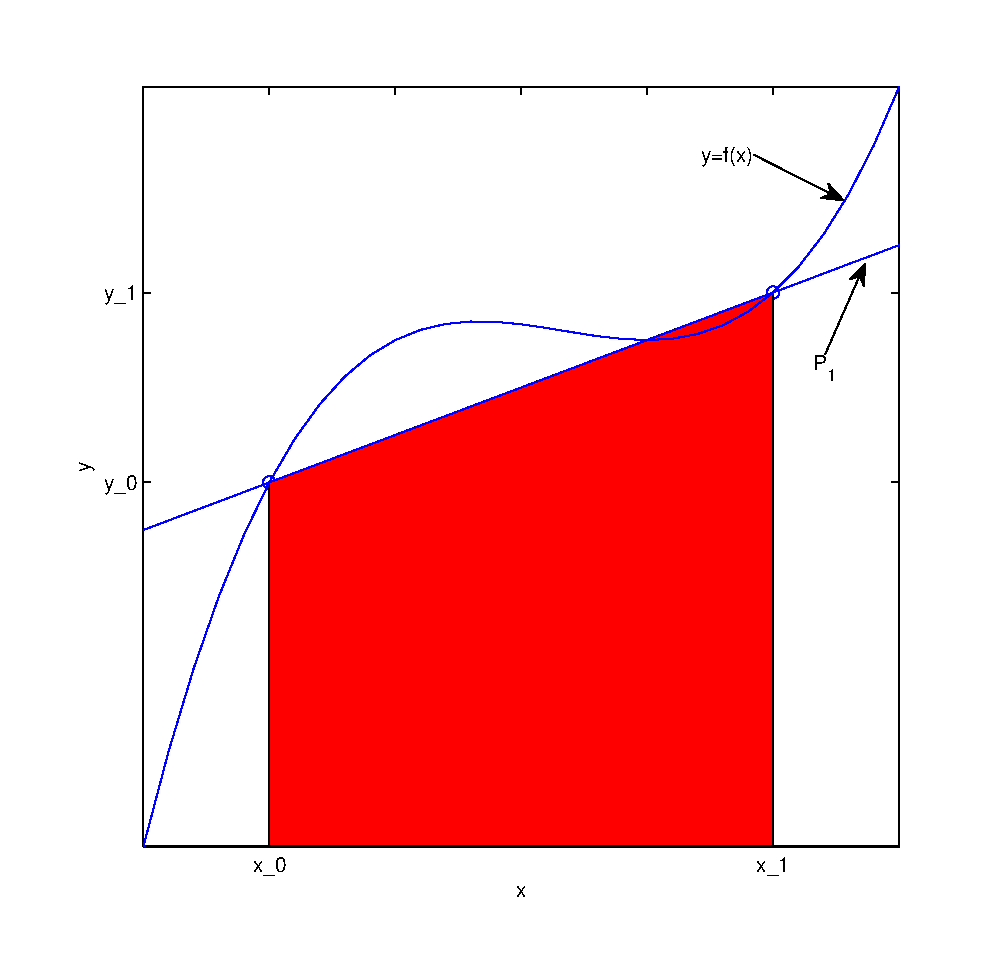
\includegraphics[width=9cm]{trapecio.eps}
\bicaption{Interpretación gráfica de la fórmula del trapecio.}{Graphical interpretation of trapezium rule.} 
\label{fig:trapecio}
\end{figure}
\begin{paracol}{2}
\paragraph*{Formula extendida (o compuesta) del trapecio.}\index{Integración! Fórmula compuesta del trapecio} La figura \ref{fig:trapecio} permite observar la diferencia entre el área calculada y el área comprendida entre la curva real y el eje $x$. Como se ha aproximado  la curva en el intervalo de integración por un línea recta (polinomio de grado 1 $p_1$), el error será tanto mayor cuando mayor sea el intervalo de integración y/o la variación de la función en dicho intervalo.

 Una solución a este problema, si se conoce la expresión analítica de la función que  se desea integrar o se conocen suficientes puntos es subdividir el intervalo de integración en intervalos más pequeños y aplicar a cada uno de ellos la fórmula de trapecio,
\switchcolumn
\paragraph{Extended (or composed) trapezium formula.} \index[eng]{Integration ! Composed trapezium formula} Figure \ref{fig:trapecio} allows us to observe the difference between the area computed and the actual area comprised between the curve and the $x$ axis. As we have approximated the curve by a straight line (1-degree interpolation polynomial $p_1$) in the integration interval, the larger the integration interval and/or the variation of the function in the interval, the larger the error we make.

One solution to this problem, if we know the analytic expression for the function we wish to integrate or we have enough points, is to divide the integration interval into shorter intervals and apply the trapezium formula in any of them.

   
\end{paracol}
\begin{equation*}
I(y)=\int_{x_0}^{x_n}ydx \approx \sum_{i=0}^{n-1}\int_{x_i}^{x_{i+1}}y(x)dx=\sum_{i=0}^{n-1}\frac{h}{2}(y_i+y_{i+1})=\frac{h}{2}\left(y_0+2y_1+2y_2+\cdots+2y_{n-1}+y_n \right)
\end{equation*}
\begin{paracol}{2}
La figura \ref{fig:trapecio2}, muestra el resultado de aplicar la fórmula extendida del trapecio a la misma función de la figura \ref{fig:trapecio}. En este caso, se ha dividido el intervalo de integración en cuatro subintervalos. Es inmediato observar a partir de la figura, que la aproximación mejorará progresivamente si se aumenta el número de subintervalos y se reduce el tamaño de los mismos.
\switchcolumn
Figure \ref{fig:trapecio2}, shows the result obtained after applying the extended trapezium formula to the same function of figure \ref{fig:trapecio}. In the present case, we have divided the integration interval into four subintervals. It is evident from the figure that the approximation will progress as the number of intervals increases and their size decreases. 
\end{paracol}
\begin{figure}[h]
\centering
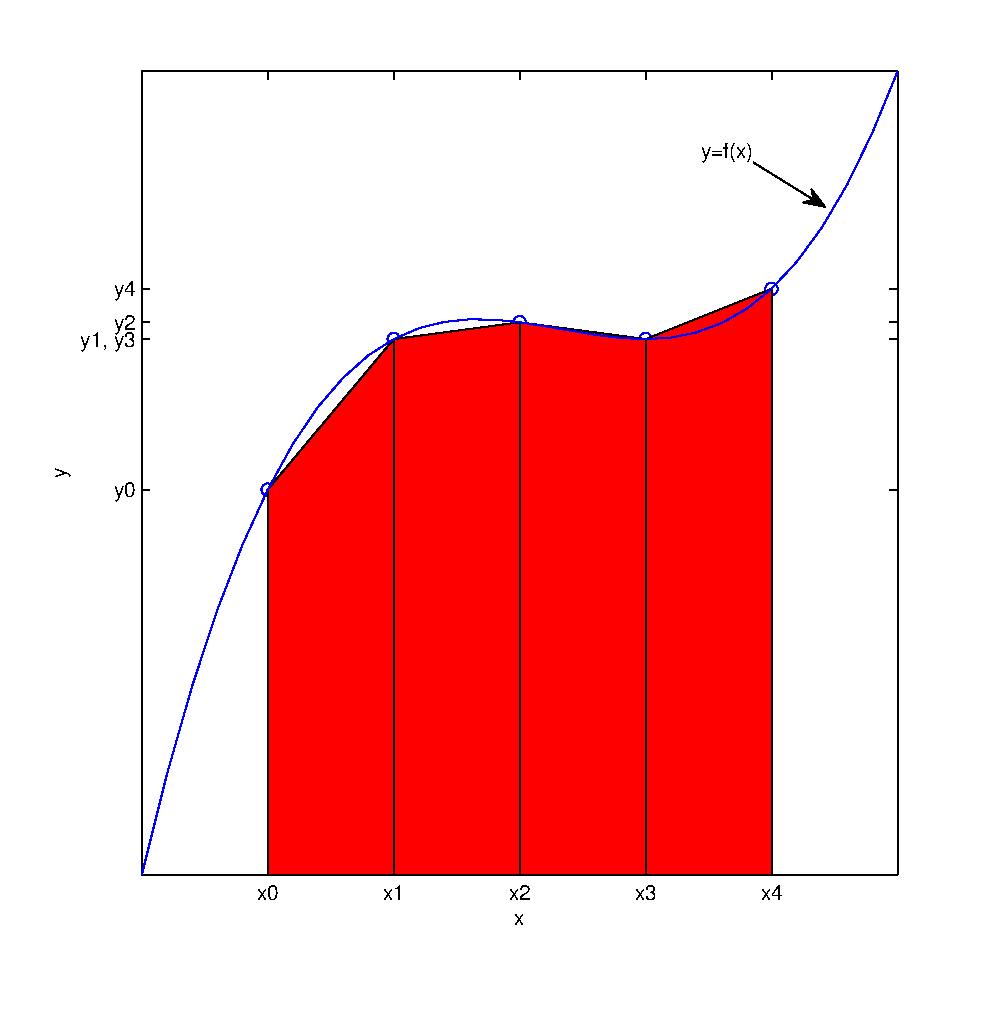
\includegraphics[width=9cm]{trapecio2.eps}
\bicaption{Interpretación gráfica de la fórmula extendida del trapecio.}{Extended trapezium formula graphical interpretation } 
\label{fig:trapecio2}
\end{figure}
\begin{paracol}{2}
\subsection{Las fórmulas de Simpson.}
Se conocen con el nombre de fórmulas integrales de Simpson, a las aproximaciones a la integral definida obtenida a partir de los polinomios interpoladores de Newton-Gregory de grado dos (Simpson $1/3$) y de grado tres (Simpson $3/8$) . \index{Integración! Fórmulas de Simpson}

En el primer caso, es preciso conocer tres valores equiespaciados de la función en el intervalo de integración y en el segundo es preciso conocer cuatro puntos. 

\paragraph*{Fórmula de Simpson $1/3$.} La fórmula de Simpson, o Simpson $1/3$,  emplea un polinomio de interpolación de Newton-Gregory de grado dos para  obtener la aproximación a la integral,

\switchcolumn
\subsection{Simpson's formulae}
The integral Simpson's formulae (or rules) are two approximations to the definite integral of a function, obtained from the Newton-Gregory's interpolation polynomials of degree two (Simpson 1/3) and degree 3 (Simpson 3/8).

In the first case we need to know three equispaced values of the function in the integration interval. In the second case we need to know four points.

\paragraph{Simpson's 1/3 formula.} The Simpson's rule or Simpson's 1/3 rule employs a 2-degree Newton-Gregory's interpolation polynomial to obtain the approximation of the integral, 
\end{paracol}
\begin{equation*}
I(y)\approx \int_{x_0}^{x_2}P_2(x)dx=\int_{x_0}^{x_2}\left(y_0+\frac{x-x_0}{h}\Delta y_0+\frac{(x-x_0)\cdot(x-x_1)}{2h^2}\Delta^2 y_0 \right)dx= \frac{h}{3}(y_0+4y_1+y_2)
\end{equation*}
\begin{paracol}{2}
La figura \ref{fig:simpsom}, muestra gráficamente el resultado de aplicar el método de Simpson a la misma función de los ejemplos anteriores.  De nuevo, la bondad de la aproximación depende de lo que varíe la función en el intervalo.  La diferencia fundamental con el método del trapecio es que ahora el área calculada esta limitada por el segmento de parábola definido por el polinomio de interpolación empleado.
\switchcolumn
Figure, \ref{fig:simpsom} shows graphically the result of applying the Simpson's method to the same function used in previous examples. Again, the goodness of the approximation depends on the function variation in the integration interval. The main difference with the trapezium method is that the area is now bounded by the parabolic segment defined by the polynomial we have utilized.   
\end{paracol}
\begin{figure}[h]
\centering
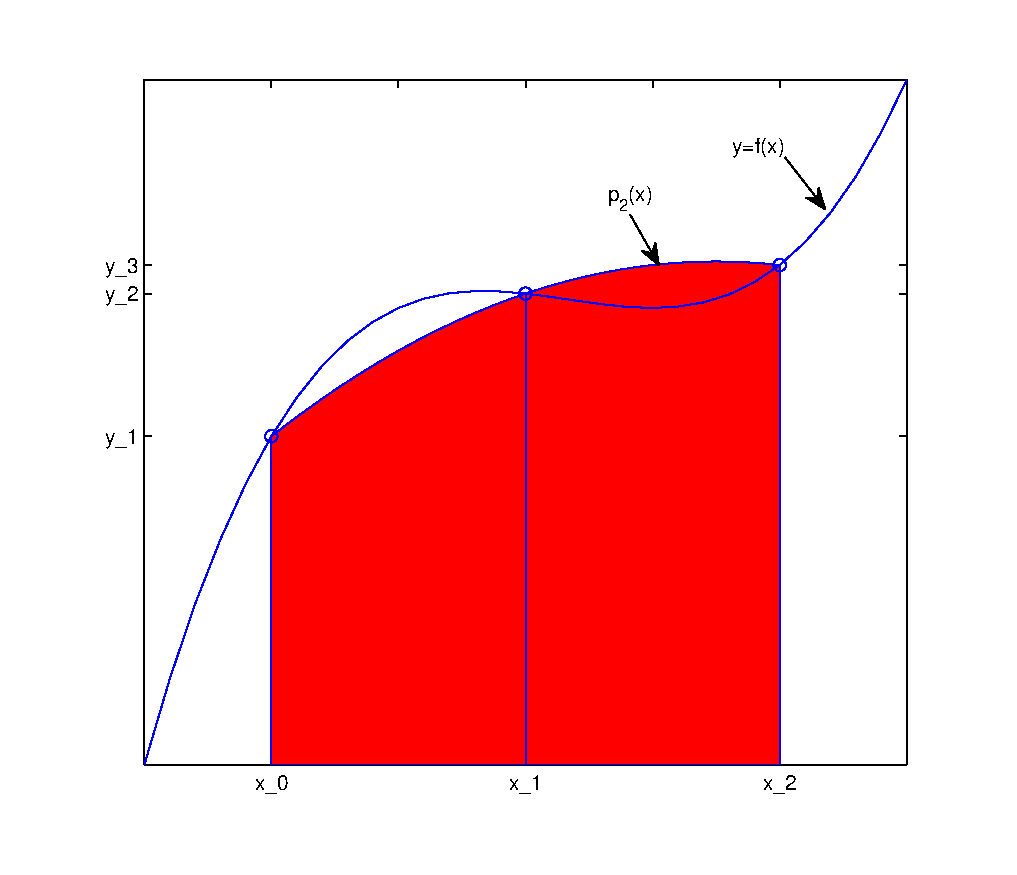
\includegraphics[width=8cm]{simpsom.eps}
\bicaption{Interpretación gráfica de la fórmula $1/3$ de Simpson.}{Graphical interpretation of Simpson's 1/3 formula} 
\label{fig:simpsom}
\end{figure}

\begin{paracol}{2}
\paragraph*{Fórmula de Simpson $3/8$.} En este caso, se emplea un polinomio de Newton-Gregory de grado 3 para obtener la aproximación a la integral,
\switchcolumn
\paragraph{Simpson's 3/8 Formula.} In this case, we use a Newton-Gregory's polynomial of degree 3 to obtain the approximation for the integral. 
\end{paracol}
\begin{align*}
I(y)&\approx \int_{x_0}^{x_3}P_2(x)dx=\\
&=\int_{x_0}^{x_3}\left(y_0+\frac{x-x_0}{h}\Delta y_0+\frac{(x-x_0)\cdot(x-x_1)}{2h^2}\Delta^2 y_0 +\frac{(x-x_0)\cdot(x-x_1)\cdot (x-x_2)}{3!h^3}\Delta^3 y_0\right)dx\\
&= \frac{3h}{8}(y_0+3y_1+3y_2+y_3)
\end{align*}

\begin{paracol}{2}
La figura  \ref{fig:simpsom38} muestra el resultado de aplicar la fórmula de Simpson $3/8$ a la misma función de los ejemplos anteriores. En este caso, la integral sería exacta porque la función de ejemplo elegida es un polinomio de tercer grado y coincide exactamente con el polinomio de interpolación construido para obtener la integral.
\switchcolumn
Figure \ref{fig:simpsom38} shows the result of applying Simpson's $3/8$ formula to the same function utilized in previous examples. In this case, the integral is exact because the example function is a three degree polynomial and fit exactly the interpolating polynomial we have built to compute the integral.
\end{paracol}
\begin{figure}[h]
\centering
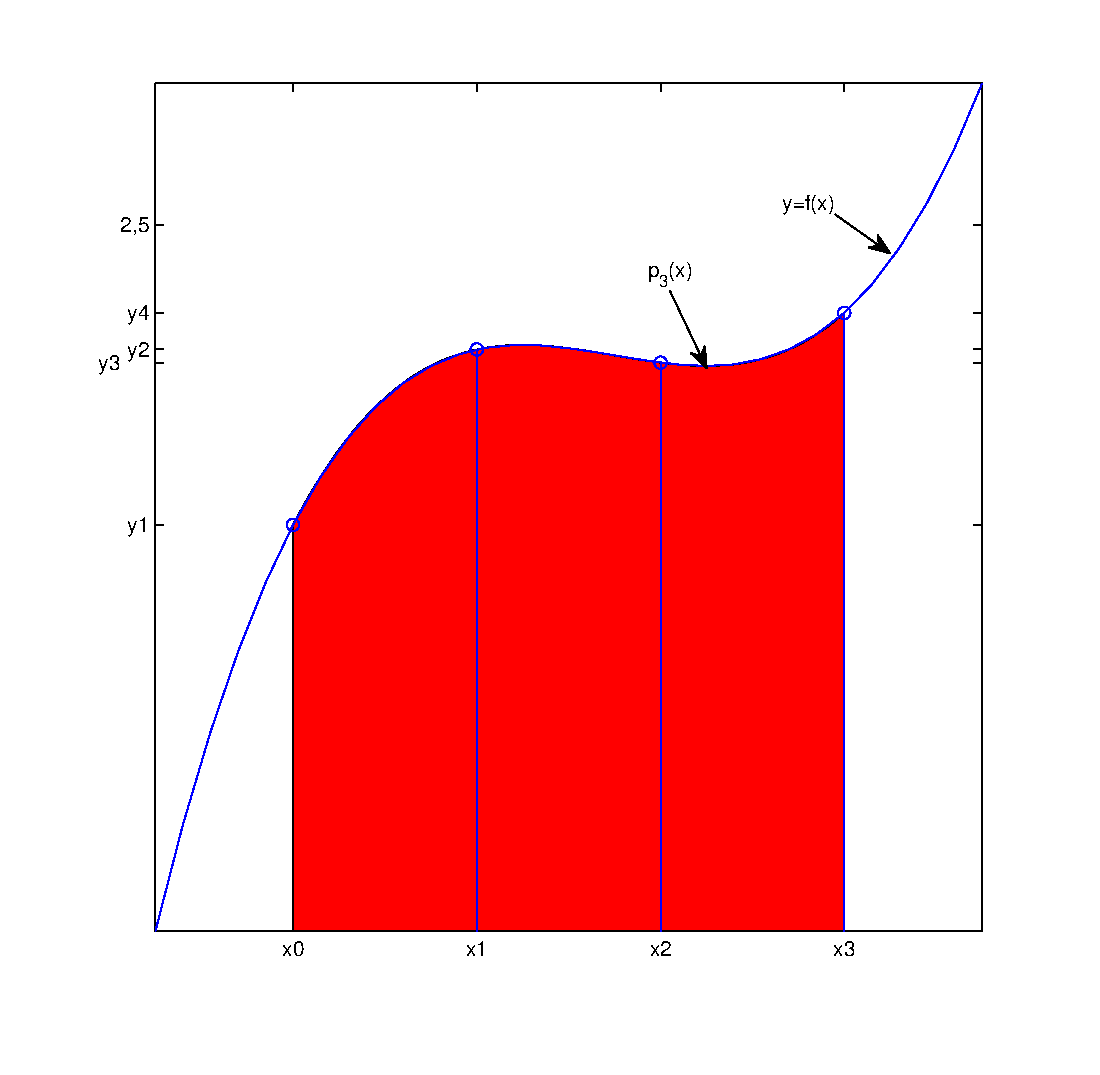
\includegraphics[width=9cm]{simpsom38.eps}
\bicaption{Interpretación gráfica de la fórmula $3/8$ de Simpson.}{Graphical interpretation of Simpson's 3/8 formula} 
\label{fig:simpsom38}
\end{figure}
\begin{paracol}{2}
Al igual que en el caso del método del trapecio, lo normal no es aplicar los métodos de Simpson a todo el intervalo de integración, sino dividirlo en subintervalos más pequeños y aplicar el método sobre dichos subintervalos. El resultado se conoce como métodos extendidos de Simpson. Al igual que sucede con la fórmula del trapecio, los métodos extendidos de Simpson mejoran la aproximación obtenida para la integral tanto más cuanto más pequeño es el tamaño de los subintervalos empleados. 

Así, la fórmula extendida de Simpson $1/3$ toma la forma,

\switchcolumn
Like the trapezium formula, we hardly ever apply Simpson's methods to the whole integration interval. Instead, we divide the integration interval into smaller subintervals and apply the method to such subintervals. The results are known as extended Simpson's methods. As in the case of the trapezium formula, the extended Simpson's methods improve the approximation computed for the integral as much as the smaller the size of the subinterval we use.

So the extended Simpson 1/3 formula takes the form,
\end{paracol}
\begin{align*}
	I(y)&\approx \sum_{i=0}^{\frac{n}{2}-1}\int_{x_{2i}}^{x_{2i+2}}P_2(x)dx=\sum_{i=0}^{\frac{n}{2}-1}\frac{h}{3}(y_{2i}+4y_{2i+1}+y_{2i+2})\\
&= \frac{h}{3}(y_0+4y_1+2y_2+4y_3+2y_4+\cdots + 2y_{n-2}+4y_{n-1}+y_n)
\end{align*}
\begin{paracol}{2}
Donde se ha dividido el intervalo de integración en $n$ subintervalos, la fórmula de Simpson se ha calculado para cada dos subintevalos y se han sumado los resultados.

Por último para la fórmula extendida de Simpson $3/8$ se puede emplear la expresión,
\switchcolumn
Where we have divided the integration interval in $n$ subintervals, the Simpson's formula has been applied to every two consecutive subintervals and, eventually we have summed the results together.
\end{paracol}
\begin{align*}
	I(y)&\approx \sum_{i=0}^{\frac{n}{3}-1}\int_{x_{3i}}^{x_{3i+3}}P_3(x)dx=\sum_{i=0}^{\frac{n}{3}-1}\frac{3h}{8}(y_{3i}+3y_{3i+1}+3y_{3i+2}+y_{3i+3})\\
&= \frac{3h}{8}(y_0+3y_1+3y_2+2y_3+3y_4+3y_5+2y_6+ \cdots + 2y_{n-3}+3y_{n-2}+3y_{n-1}+y_n)
\end{align*}
\begin{paracol}{2}
En este caso también se divide el intervalo en $n$ subintervalos pero ahora se ha aplicado la regla de Simpson $3/8$ a cada tres subintevalos.

A continuación se incluye un código que permite permite aproximar la integral definida de una función en un intervalo por cualquiera de los tres métodos descritos: Trapecio, Simpson o Simpson $3/8$,
\switchcolumn
In this case, we have also divided the interval in $n$ subintervals but now we apply the Simpson's 3/8 rule to each group of three successive subintervals.

The code included below compute an approximation to de definite integral of a function using any one the three method we have described: Trapezium, Simpson's or Simpson's 3/8, 
\end{paracol}
\inputminted[
frame=lines,
framesep=2mm,
baselinestretch=1.2,
%bgcolor=LightGray,
label=integrador.py,
fontsize=\footnotesize,
linenos
]{python}{./codigos/diferenciacion_integracion/integrador.py}

\begin{paracol}{2}
Este programa contiene dos funciones. La primera \mintinline{python}{integra } aplica directamente el método deseado sobre el intervalo de integración. Para obtener los métodos extendidos, podemos emplear la segunda función \mintinline{python}{trocea} que divide el intervalo de integración inicial en el número de subintervalos que deseemos, apliqua el programa anterior a cada subintervalo, y, por último, suma todo los resultados para obtener el valor de la integral en el intervalo deseado.

Por último, indicar que el modulo de Py\-thon, Scipy  posee varias funciones para calcular la integral definida de una función. Se encuentran dentro del submódulo \mintinline{python}{integrate}. Para calcular la integral definida de una función lo más sencillo es usar el comando\\ \texttt{integrate.quad}. Este comando admite como variables de entrada el nombre de una función, y dos valores que representan los límites de integración. Como variable de salida devuelve el valor de la integral definida en el intervalo introducido y una estimación del error cometido. El siguiente código muestra un ejemplo de uso de la función \mintinline{python}{quad} y compara los resultados con la funcion \mintinline{python}{trocea} cuyo código hemos incluido más arriba.
\switchcolumn
This program holds two functions. The first one \mintinline{python}{integra} applies the method directly over the integration interval. To obtain the extended methods, we can employ the second included function \mintinline{python}{trocea}, which divides the initial integration interval into the number of subintervals we wish, applies the function \mintinline{python}{integra} to any subinterval and, eventually, add all the results together to obtain the value of the integral in the wished interval.

Lastly, the Python module Scipy has several functions to compute a function's definite integral. It is located in the submodule \mintinline{python}{integrate}. The easiest way To compute the integral of a function is to use the function \mintinline{python}{integrate.quad}. This function takes a funtion name and two variables which represent the integration limits as imputs and returns the integral value in the interval introduced and an estimation of the committed error. The following code shows a use example of the function \mintinline{python}{quad} and compares the results with those of the function \mintinline{python}{trocea} whose code we have included above. 
\end{paracol}

\begin{minted}{python}
In [56]: import scipy.integrate as integ

In [57]: def probando(x):
...:     """test funtion to be integrate"""
...:     return((x-1)*x*(x-2))+6
...:     

In [58]: inte.quad(probando,-5,2.5)
Out[58]: (-260.85937499999994, 3.3240810849038596e-12)

In [59]: trocea(probando,'simpson',[-5,2.5],5)
Out[59]: -260.859375
\end{minted}

\begin{paracol}{2}
\section{Problemas de valor inicial en ecuaciones diferenciales}
\sectionmark{Problemas de valor inicial. \textreferencemark\ Initial value problems.}
Las leyes de la física están escritas en forma de ecuaciones diferenciales. \index{Ecuación diferencial} \index{Problemas de valor inicial}

Una ecuación diferencial establece una relación matemática entre una variable y sus derivadas respecto a otra u otras variables de las que depende. El ejemplo más sencillo lo encontramos en las ecuaciones de la dinámica en una sola dimensión que relacionan la derivada segunda de la posición de un cuerpo con respecto al tiempo, con la fuerza que actúa sobre el mismo.
\switchcolumn
\section{Differential equations. Initial value problems}
The laws of physics are written as differential equations \index[eng]{Differential equation}\index[eng]{Initial value problems.}

Differential equations establish a mathematical relationship between a variable and its derivatives with respect to another variable or other variables the first variable depends upon. We can find the simplest example watching the one dimensional dynamics equations which link the second derivative of a body position with the force acting on the body.  
\end{paracol}
\begin{equation*}
m\cdot \frac{d^2x}{dt^2}=F
\end{equation*}
\begin{paracol}{2}
Si la fuerza es constante, o conocemos explícitamente como varía con el tiempo, podemos integrar la ecuación anterior para obtener la derivada primera de la posición con respecto al tiempo ---la velocidad--- de una forma directa,

\switchcolumn
If the force applied is constant or we know explicitly how it evolves on time, we can integrate the previous equation to straightforwardly obtain the position first derivative with respect to time ---the velocity---,
\end{paracol}
\begin{equation*}
m\cdot \frac{d^2x}{dt^2}=F \rightarrow v(t)=\frac{dx}{dt}=\int \frac{F(t)}{m}dt +v(0)
\end{equation*}
\begin{paracol}{2}
Donde suponemos conocido el valor $v(0)$ de la velocidad del cuerpo en el instante inicial.

Si volvemos a integrar ahora la expresión obtenida para la velocidad, obtendríamos la posición en función del tiempo,

\switchcolumn
When we consider we know the body velocity $v(0)$ at the initial time.

If we now integrate the expression we have got for the the velocity, we obtain the position as a function of time,
\end{paracol}
\begin{equation*}
v(t)=\frac{dx}{dt}=\int \frac{F(t)}{m}dt +v(0)\rightarrow x(t)=\int\left(\int \frac{F(t)}{m}dt +v(0)\right)dt+x(0)
\end{equation*}
\begin{paracol}{2}
Donde suponemos conocida la posición inicial $x(0)$.

Quizá el sistema físico idealizado más conocido y estudiado es el oscilador armónico. En este caso, el sistema está sometido a una fuerza que depende de la posición y, si existe disipación, a una fuerza que depende de la velocidad,

\switchcolumn
Were we suppose the initial position $x(0)$ is known.

Perhaps the better known and most studied physical idealised system is the harmonic oscillator. In this case, the system suffers a force that depends on the position and, if the oscillator is damped, it suffer also a force that depends on the speed,  

\end{paracol}
\begin{equation*}
m\frac{d^2x}{dt^2}=-kx-\mu \frac{dx}{dt}
\end{equation*}
\begin{paracol}{2}
En este caso, la expresión obtenida constituye una ecuación diferencial ordinaria y ya no es tan sencillo obtener una expresión analítica para $x(t)$. Para obtener dicha expresión analítica, es preciso emplear métodos de resolución de ecuaciones diferenciales.

El problema del oscilador armónico, pertenece a una familia de problemas conocida como problemas de valores iniciales. En general, un problema de valores iniciales de primer orden consiste en obtener la función $x(t)$, que satisface la ecuación,
\switchcolumn
In this last case, the expression we obtain is an ordinary differential equation (ODE), and it is no longer so easy to solve and obtain an analytical expression for $x(t)$. To obtain such a expression we need to use specific methods to solve differential equations

The harmonic oscillator problem belongs to a problems family knows as initial value problems. In general, to solve a first order initial value problem is to obtain the function $x(t)$, that satisfies the equation, 
\end{paracol} 
\begin{equation*}
x'(t)\equiv \frac{dx}{dt}=f(x(t),t), \ x(t_0)
\end{equation*}
\begin{paracol}{2}
Donde $x(t_0)$ representa un valor inicial conocido de la función $x(t)$.

En muchos casos, las ecuaciones diferenciales que describen los fenómenos físicos no admiten una solución analítica, es decir no permiten obtener una función para $x(t)$. En estos caso, es posible obtener soluciones numéricas empleando un computador. El problema de valores iniciales se reduce entonces a encontrar un aproximación discretizada de la función $x(t)$. 

El desarrollo de técnicas de integración nu\-mérica de ecuaciones diferenciales constituye uno de los campos de trabajo más importantes de los métodos de computación científica. Aquí nos limitaremos a ver los más sencillos.

Esencialmente, los métodos que vamos a describir se basan en discretizar el dominio donde se quiere conocer el valor de la función $x(t)$. Así por ejemplo si se quiere conocer el valor que toma la función en el intervalo $t \in [a,b]$, se divide el intervalo en $n$ subintervalos cada uno de tamaño $h_i$. Los métodos que vamos a estudiar nos proporcionan una aproximación de la función $x(t)$, $x_0,x_2\cdots x_n$ en los $n+1$ puntos $t_0,t_1,\cdot, t_n$, donde $t_0=a$, $t_n=b$, y $t_{i+1}-t_i=h_i$. El valor de $h_i$ recibe el nombre de paso de integración. Además se supone conocido el valor que toma la función $x(t)$ en el extremo inicial $a$, $x(a)=x_a$.
  
\subsection{El método de Euler.}
El método de Euler, puede obtenerse a partir del desarrollo de Taylor de la función $x$, entorno al valor conocido $(a,x_a)$. La idea es empezar en el valor conocido e ir obteniendo iterativamente el resto de los valores $x_1,\cdots$ hasta llegar al extremos $b$ del intervalo en que queremos conocer el valor de la función $x$. En general podemos expresar la relación entre dos valores sucesivos a partir del desarrollo de Taylor como, \index{Método de Euler}
\switchcolumn
Where $x(t_0)$ represents a known initial value of the function $x(t)$.

In many cases, differential equations describe physical phenomena that not have an analytical solution. That is, there in no analytical function $x(t)$ that satisfies de differential equation. In these cases is still possible to compute numerical solutions using a computer. The initial value problems reduces then to find  a discretised version of the function $x(t)$.

Developing techniques to numerically solve differential equations is perhaps one of the most important fields of scientific computing. Here, we will describe only me most basic me\-thods.

The methods we are going to introduce are essentially base on discretising the domain in which we want to know the value of the function $x(t)$. For instance, If we want to know the values of the function in the interval $t \in [a,b]$, we divide the interval in $n$ subinterval, each one of size $h_i$. The methods qe are going to study give us an approximation of the function $x(t)$, $x_0,x_2\cdots x_n$ in the $n+1$ points $t_0,t_1,\cdot, t_n$, where $t_0=a$, $t_n=b$, y $t_{i+1}-t_i=h_i$. The value $h_i$ is known as the integration step. Besides, we suppose that we know the value the function $x(t)$ takes in the interval initial side $a$, $x(a) = x_a$.

\subsection{The Euler's method.}
The Euler's method can be obtained from the Taylor's expansion of the function $x$, around the known value $(a,x_a)$. The idea is to start at the known value an compute iteratively the remaining values $x_1\cdots$ until we arrive to the end of the interval $b$, at which we want to know the value function $x$ takes.

We can obtain the relationship between to consecutive values of the function from the Taylor's expansion as, 
\end{paracol}
\begin{equation*}
x(t_{i+1})=x(t_i)+(t_{i+1}-t_{i})x'(t_i)+\frac{(t_{i+1}-t_{i})^2}{2}x''(t_i)+\cdots+ \frac{(t_{i+1}-t_i)^n}{n!}x^{(n)}(t_i)+\cdots
\end{equation*}
\begin{paracol}{2}
Como se trata de un problema de condiciones iniciales, conocemos la derivada primera de la función $x(t)$, explícitamente,$x'(t)=f(x(t),t)$. Por tanto podemos sustituir las derivadas de $x$ por la función $f$ y sus derivadas con respecto a t,
\switchcolumn
As we are solving an initial condition problem, we know first the derivative of function $x(t)$ at the initial point $x'(t) = f(x(t),t)$. Therefore, we may substitute  the derivatives of $x$ by the funtion $f$ an its derivatives with respect to t.
\end{paracol}
\begin{equation*}
x(t_{i+1})=x(t_i)+(t_{i+1}-t_{i})f(t_i,x_i)+\frac{(t_{i+1}-t_{i})^2}{2}f'(t_i,x_i)+\cdots+ \frac{(t_{i+1}-t_i)^n}{n!}f^{(n-1)}(t_i,x_i)+\cdots
\end{equation*}
\begin{paracol}{2}
Donde $x_i\equiv x(t_i)$. Si truncamos el polinomio de Taylor, quedándonos solo con el término de primer grado, y hacemos que el paso de integración sea fijo, $h_i\equiv h=\mathrm{cte}$ obtenemos el método de Euler,
\switchcolumn	
Where $x_i\equiv x(t_i)$. If we truncate the Taylor's polynomial, leaving only the first order term and set the integration step to a constant value, $h_i \equiv h = cte$ we arrive to the Euler's method,
\end{paracol}
\begin{equation*}
x_{i+1}=x_i+h\cdot f(t_i,x_i)
\end{equation*}
\begin{paracol}{2}
A partir de un valor inicial, $x_0$ es posible obtener valores sucesivos mediante un algoritmo iterativo simple,
\switchcolumn
Departing from a known initial value, $x_0$, we can obtain the successive values using a simple iterative algorithm,
\end{paracol}
\begin{align*}
x_0&=x(a)\\
x_1&=x_0+hf(a,x_0)\\
x_2&=x_1+hf(a+h,x_1)\\
\vdots \\
x_{i+1}&=x_i+hf(a+ih,x_i)
\end{align*}
\begin{paracol}{2}
El siguiente código implementa el método de Euler para resolver un problema de condiciones iniciales de primer orden a partir de una función $f(t)$ y un valor inicial $x_0$.
\switchcolumn
The following code implements the Euler's method using a function $f(t)$ and an initial value $x_0$ as inputs,
\end{paracol}
\inputminted[
frame=lines,
framesep=2mm,
baselinestretch=1.2,
%bgcolor=LightGray,
label=Euler\_method.py,
fontsize=\footnotesize,
linenos
]{python}{./codigos/diferenciacion_integracion/Euler_method.py}

\begin{paracol}{2}
Un ejemplo sencillo de problema de condiciones iniciales de primer orden, nos los suministra la ecuación diferencial de la carga y descarga de un condensador eléctrico. La figura \ref{fig:RC}, muestra un circuito eléctrico elemental formado por una resistencia $R$ en serie con un condensador $C$. \index{Circuito RC}
\switchcolumn
The differential equation that models the charge and discharge of an electronic capacitor supplies a simple example of an first order initial condition problem. Figure \ref{fig:RC} shows a electronic circuit composed of a resistor $R$ in series with a capacitor $C$. \index[eng]{RC circuit}
   
\end{paracol}
\begin{figure}[h]
\centering
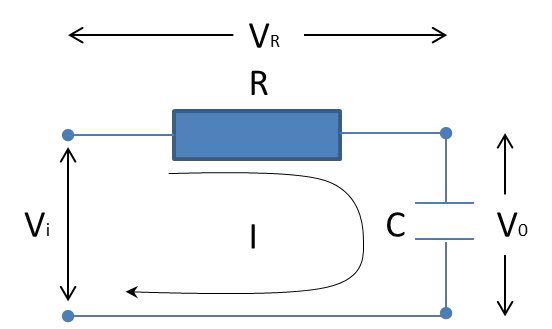
\includegraphics[width=9cm]{rc.pdf}
\caption{Circuito RC}
\label{fig:RC}
\end{figure}
\begin{paracol}{2}
La intensidad eléctrica que atraviesa un condensador depende de su capacidad, y de la variación con respecto al tiempo del voltaje entre sus extremos,
\switchcolumn	
The electric current that passes through a capacitor depends on the capacitor capacity and on the variation on time of the voltage applied to it.
 
\end{paracol}
\begin{equation*}
I=c\frac{dV_o}{dt}
\end{equation*}
\begin{paracol}{2}
La intensidad que atraviesa la resistencia se puede obtener a partir de la ley de Ohm,
\switchcolumn
the current through the resistor can be computed using Ohm's law.
\end{paracol}
\begin{equation*}
V_R=I\cdot R
\end{equation*}
\begin{paracol}{2}
Por otro lado, la intensidad que recorre el circuito es común para la resistencia y el condensador. El voltaje suministrado tiene que ser la suma de las caídas de voltaje en la resistencia y en el condensador, $V_i=V_o+V_R$. Sustituyendo y despejando,

\switchcolumn
Additionally, the current flowing through the circuit is the same for both the resistor and the capacitor. The voltage supplied to the circuit should equal the sum of the resistor and capacitor voltage drop, expressed as $V_i = V_o + V_R$. By substituting and solving,
\end{paracol}
\begin{equation*}
V_i=V_o+V_R \rightarrow V_i=V_o+I\cdot R \rightarrow V_i=V_o+R\cdot C\frac{dV_0}{dt}
\end{equation*}
\begin{paracol}{2}
Si reordenamos el resultado,
\switchcolumn
And, after rearranging the result,  
\end{paracol}
\begin{equation*}
\frac{dV_o}{dt}=\frac{V_i-V_o}{R \cdot C}
\end{equation*}
\begin{paracol}{2}
Obtenemos una ecuación diferencial para el valor del voltaje en los extremos del condensador que puede tratarse como un  problema de valor inicial. Para este problema, la función $f(t,x)$ toma la forma,
\switchcolumn
We get a differential equation for the capacitor tension drop that could be solve as a initial value problem. For this problem the function $f(t,x)$ takes the form,
\end{paracol}
\begin{equation*}
f(t,V_0 \equiv x) = \frac{V_i-V_o}{R \cdot C}
\end{equation*}
\begin{paracol}{2}
Además necesitamos conocer un valor inicial $V_o(0)$ para el voltaje en el condensador. Si suponemos que el condensador se encuentra inicialmente descargado, entonces $V_o(0)=0$. Para este problema se conoce la solución analítica. El voltaje del condensador en función del tiempo viene dado por la función,
\switchcolumn
In addition, we need to know an initial value $V_o(0)$ for the voltage across the capacitor. If we consider the capacitor is initially discharged, then $V_o(0) = 0$. For this problem we know the analytic solution. We can express the voltage across the capacitor as a function fo time,
\end{paracol}
\begin{equation*}
V_0(t)=V_i\left(1-e^{-t/R\cdot C}\right)
\end{equation*} 

\begin{paracol}{2}
Podemos resolver el problema de la carga del condensador, empleando la función  \mintinline{python}{Euler} incluida más arriba. Lo único que necesitamos es definir una función en Python  para representar la función $f(x,t)$ de nuestro problema de valor inicial,
\switchcolumn
We can solve the capacitor problem using the function \mintinline{python}{euler} included above. WE only need to define a Python funtion to represent the funtion $f(x,t)$ for our initial value problem,
\end{paracol}
%\begin{lstlisting}
\begin{minted}{python}
	In [151]: def condensador(t,Vo,C=1.,R=1.,Vi=10.):
	...:     dVo = (Vi-Vo)/(R*C)
	...:     return(dVo)
\end{minted}

\begin{figure}[h]
\centering
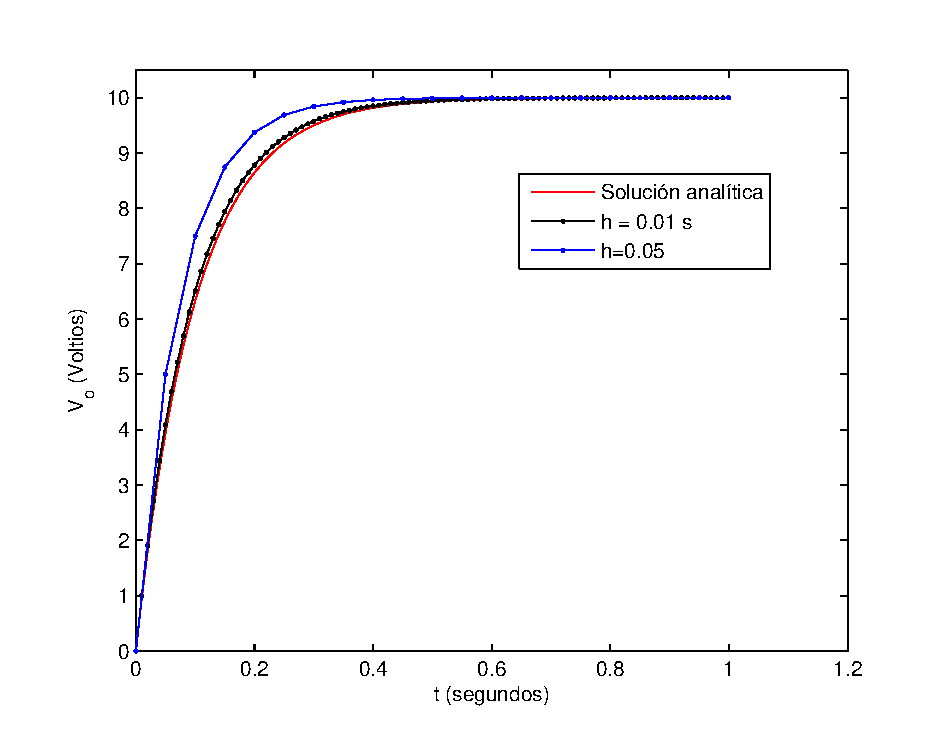
\includegraphics[width=12cm]{solrc.eps}
\bicaption{Comparacion entre los resultados obtenidos mediante el método de Euler para dos pasos de integración $h=0.5$ y $h=0.25$ y la solución analítica para el voltaje $V_o$ de un condensador durante su carga. Hemos tomado $C=R=1$ y $V_i=10$}{Comparison among the results obtained using Euler's method with two different integration steps $h=0.5$ y $h=0.25$, and the analytic solution for voltage $V_o$ across a capacitor. We took $C=R=1$ and $V_i=10$.}
\label{fig:solrc}
\end{figure}
\begin{paracol}{2}
La figura \ref{fig:solrc} compara gráficamente los resultados obtenidos si empleamos la función\\ \texttt{euler(condensador,0,0,10,h)}, para obtener el resultado de aplicar al circuito un voltaje de entrada constante $V_i=10$V durante 10 segundos, empleando dos pasos de integración distintos $h=0.5$s  y $h=0.025$s. Además, se ha añadido a la gráfica el resultado analítico.

En primer lugar, es interesante observar como el voltaje $V_0$ crece hasta alcanzar el valor $V_i=10$ V del voltaje suministrado al circuito. El tiempo que tarda el condensador en alcanzar dicho voltaje y quedar completamente cargado depende de su capacidad y de la resistencia presente en el circuito.

Como era de esperar, al hacer menor el paso de integración la solución numérica se aproxima más a la solución analítica. Sin embargo, como pasaba en el caso de los métodos de diferenciación de funciones, hay un valor de $h$ óptimo. Si disminuimos el paso de integración por debajo de ese valor, los errores de redondeo empiezan a dominar haciendo que la solución empeore.

\paragraph{Problema de segundo orden.} Vamos a considerar ahora un sistema con una masa colgada de un resorte con un dispositivo mecánico (amortiguador) que ejerce una fuerza opuesta al movimiento proporcional a la velocidad. En este caso la ecuación diferencial sería la siguiente:

\switchcolumn
Figure \ref{fig:solrc} graphically compares the results achieved using the function\\ \texttt{euler(condensador,0,0,10,h)} to compute the voltage across the capacitor after supplying a constant input voltage $V_i = 10V$ during ten seconds, using two different integration steps, $h=0.5s$ ans $h=0.25s$. We have also added the analytical solution to the problem to the graphic. 

It's interesting to observe how the voltage, denoted as $V_0$, increases until it reaches the value $V_i = 10V$, which corresponds to the voltage supplied to the circuit. The time it takes for the capacitor to reach this voltage and become fully charged depends on its capacitance and the value of the resistor in the circuit.

As expected, when we diminish the integration step, the numerical solution approximates the analytical solution better. However, as we saw for the case of numerical differentiation, there is an optimal $h$. If we take the integration step value below this optimal value, the round-off errors worsen the solution.

\paragraph{a Second-order problem.} Let's consider now a system with a mass hanging of a spring and with a mechanical gadget (damper) that exerts a force  opposite to the mass movement and proportional to the mass speed. For this system the differential equation is as follows:

\end{paracol}

\begin{equation*}
m\frac{d^2 y}{dt^2}=m\cdot g-k \cdot y-\mu \frac{dy}{dt}
\end{equation*}

\begin{figure}[h]
	\centering
	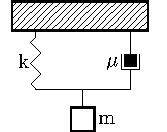
\includegraphics[width=6cm]{figura_amortiguador.pdf}
	\bicaption{Masa suspendida en vertical de un muelle con rozamiento.}{A mass vertically hanging of a sprint with a damping resistance}.
	\label{fig:masa_suspendida}
\end{figure}

\begin{paracol}{2}
Tenemos un problema de valor inicial de segundo orden, con una ecuación en la que conviven la variable $y$ su derivada $\frac{dy}{dt}$ y su derivada segunda $\frac{d^2y}{dt^2}$. Para resolver este tipo de problemas lo que hacemos es reescribir la ecuación como dos ecuaciones de primer orden, una para la posición $y$ y otra para la velocidad $v_y=\frac{dy}{dt}$ de manera que obtendríamos un sistema de dos ecuaciones de primer orden acopladas:
\switchcolumn
We have a second-order initial values problem, with an equation that links the variable $y$ its first derivative $\frac{dy}{dt}$ and its second derivative $\frac{d^2y}{dt^2}$. To solve this kinda problem, we rewrite the differential equation using  two first-order differential equations. one for the position $y$ and the other for the velocity $v_y = \frac{dx}{dt}$. IN this way, we obtain two coupled first-order equations:    
\end{paracol}
\begin{align*}
\frac{dy}{dt}&=v_y \\
\frac{dv_y}{dt}&=g-\frac{k}{m}\cdot y - \frac{\mu}{m}\cdot v_y 
\end{align*}

\begin{paracol}{2}
Ese sistema de ecuaciones de primer orden se puede resolver usando el método de Euler. Necesitamos definir una función de Python para representar el sistema de ecuaciones diferenciales,

\switchcolumn
This system can be solve using the Euler's method, but we need to define a Python function to represent the system of differential equations,
\end{paracol}

\begin{minted}{python}
	def amortiguador(t,y):
	"""
	Defines the set of differetial equations for a damping
	oscilator 
	
	Parameters
	----------
	t : TYPE double 
	DESCRIPTION. time
	y : TYPE numpy array
	DESCRIPTION. y[0] ->> position
	y[1] ->> velocity
	
	Returns
	-------
	dydt : TYPE numpy arra
	DESCRIPTION. dydt[0] ->> velocity
	dydt[1] ->> acceleration
	
	"""
	g = 9.8 #gravity accel.
	k = 100. #spring constant
	m = 2.  #mass
	mu = 0.5 #friction constant
	dydt = np.zeros(2) 
	dydt[0]=y[1]
	dydt[1]=g-(k/m)*y[0]-(mu/m)*y[1];
	return(dydt)
\end{minted}

\begin{paracol}{2}
Empleando la función descrita \\ \texttt{euler('amortiguador',[0 0],0,50,0.01)} obtenemos la evolución temporal de la posición y la velocidad de la masa unida al resorte como puede verse en la figura \ref{fig:amortiguador1}. En esta figura se aprecia como la masa oscila en torno a la posición de equilibrio hasta que finalmente se para.
\switchcolumn
Using the function just described \\ \texttt{euler('amortiguador',[0 0],0,50,0.01)} we compute the temporal evoluntion of position and velocity for the mass attached to the spring. Figure \ref{fig:amortiguador1} shows the result, the mass oscillates around an equilibrium position until the damping mechanism, eventually, stops it. 
\end{paracol}
\begin{figure}[h]
	\centering
	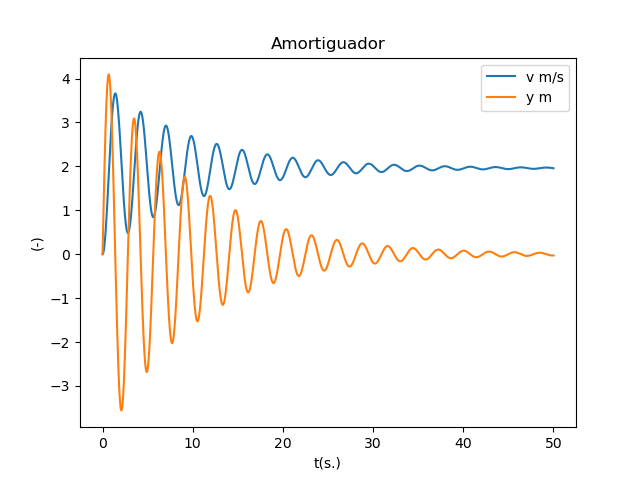
\includegraphics[width=12cm]{amortiguador_1.png}
	\bicaption{Resultado de aplicar el método de Euler a una masa suspendida en vertical de un muelle con rozamiento.}{Results achieved using Euler's method to solve the damped oscillator problem.}
	\label{fig:amortiguador1}
\end{figure}
\begin{paracol}{2}
Si cambiamos el valor de la constante del muelle a $k=100$ ($kg/s^2$) y volvemos a aplicar el método de Euler para resolver obtenemos el resultado mostrado en la figura \ref{fig:amortiguador2}. En la gráfica puede observarse que la masa comienza a oscilar con oscilaciones de amplitud creciente. Para analizar este comportamiento anómalo vamos a repetir el método de Euler reduciendo en un orden de magnitud el paso de integración. Si lo hacemos así obtenemos los resultados de la figura \ref{fig:amortiguador3}. Al reducir el paso vemos que la masa oscila en torno a la posición de equilibrio hasta que se estabiliza. El comportamiento observado en la figura \ref{fig:amortiguador2} se debe a errores de integración del algoritmo de Euler.
\switchcolumn
If we change the values of the spring constant to $k=100$ ($kg/s^2$) and repeat the Euler's method, we arrive to the results showed figure \ref{fig:amortiguador2}. We can see in the graphic how the mass oscillates with increasing oscillation amplitude. To analyse this unexpected result we are going to repeat the Euler's method computing, this time using an integration step one order of magnitude less. We obtain for this new calculation the behaviour showed in figure \ref{fig:amortiguador3}. Notice how reducing the integrations step reverts the situation and now, the solution of the problem is reasonable, the mass oscillations diminish until, eventually, it stops. The behaviour observed in figure \ref{fig:amortiguador2} is due to Euler's method integration error.   
\end{paracol}
\begin{figure}[h]
	\centering
	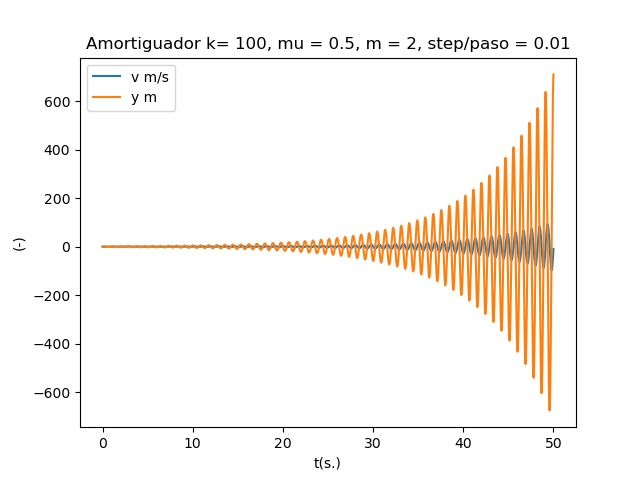
\includegraphics[width=12cm]{amortiguador_2.png}
	\bicaption{Resultado de aplicar el método de Euler a una masa suspendida en vertical de un muelle con rozamiento $k=100$.}{Result achieved using Euler's method to solve the damped oscillator problem. $K=100$}
	\label{fig:amortiguador2}
\end{figure}

\begin{figure}[h]
	\centering
	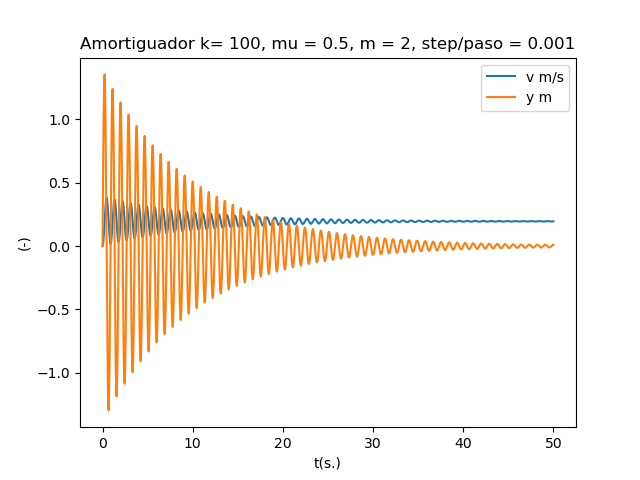
\includegraphics[width=12cm]{amortiguador_3.png}
	\bicaption{Resultado de aplicar el método de Euler a una masa suspendida en vertical de un muelle con rozamiento $k=100$ y paso $h=0.001$.}{Result achieved using Euler's method to solve the damped oscillator problem. $K=100$, $h = 0.001$}
	\label{fig:amortiguador3}
\end{figure}
\begin{paracol}{2}
En la práctica se emplean algoritmos más precisos (y complejos) que el de Euler para resolver problemas de valor inicial, por ejemplo los métodos de Runge-Kutta.
\switchcolumn
In practice, there are more precise (an complex) algorithms than Euler's to solve initial value problems. For instance, the family of Runge-Kutta methods.
\end{paracol}
\begin{flalign*}
	&\mathwitch*_{i=0}^{\infty} \Biggl \{&     
\end{flalign*}

\begin{paracol}{2}

\subsection{Métodos de Runge-Kutta} \index{Método de Runge-Kutta}
Si intentamos emplear polinomios de Taylor de grado superior, al empleado en el método de Euler, nos encontramos con la dificultad de obtener las derivadas sucesivas, de la función $f$. Así, si quisiéramos emplear el polinomio de Taylor de segundo grado, para la función $x$, tendríamos,

\switchcolumn
\subsection{The Runge-Kutta methods}\index[eng]{RUnge-Kutta methods}
If we try to use Taylor's polynomials of higher degree than that used in Euler's method, we have the find the problem of computing the successive derivatives of the function $f$. So if we want to use the Taylor's second-degree polynomial, to compute the values of $x$, we have,   
\end{paracol}  
\begin{equation*}
x(t_{i+1})=x(t_i)+h\cdot f(t_i,x_i)+\frac{h^2}{2}f'(t_i,y_i)
\end{equation*}
\begin{paracol}{2}
Pero,
\switchcolumn
but,
\end{paracol}
\begin{equation*}
f'(t,x)=\frac{\partial f(t,x)}{\partial t}+\frac{\partial f(t,x)}{\partial x}\cdot f(t,x)
\end{equation*}
\begin{paracol}{2}
Sacando factor común $h$, obtenemos,
\switchcolumn
Taking out common factor $h$, we get,
\end{paracol}
\begin{equation*}
x(t_{i+1})=x(t_i)+h\left(f(t_i,x_i)+\frac{h}{2}\left(\frac{\partial f(t_i,x_i)}{\partial t}+\frac{\partial f(t_i,x_i)}{\partial x}\cdot f(t_i,x_i)\right)\right)
\end{equation*}
\begin{paracol}{2}
A partir de este resultado, es fácil comprender que resulte complicado obtener métodos de resolución basados en el desarrollo de Taylor. De hecho, se vuelven cada vez más complicados según vamos empleando polinomios de Taylor de mayor grado.

Desde un punto de vista práctico, lo que se hace es buscar aproximaciones a los términos sucesivos del desarrollo de Taylor, para evitar tener que calcularlos explícitamente. Estas aproximaciones se basan a su vez, en el desarrollo de Taylor para funciones de dos variables.

Los métodos de integración resultantes, se conocen con el nombre genérico de métodos de Runge-Kutta. Veamos cómo se haría para el caso que acabamos de mostrar del polinomio de Taylor de segundo grado.

En primer lugar obtenemos el desarrollo del polinomio de Taylor de primer grado, en dos variables de la función $f(t,x)$, en un entorno del punto $t_i,x_i$,
\switchcolumn
This result clearly shows that developing methods for solving initial value problems based on Taylor's expansion is challenging. In fact, it becomes increasingly complex as we employ Tailor's polynomials of a higher degree.

From a practical point of view, the common practice is to search for approximations to successive Taylor's expansion terms rather than calculate them explicitly. These approximation are, in turn, based on Taylor's expansion for two variable functions.

The resulting methods are known in general as the Runge-Kutta methods. Let us see how to do it for the case we have just shown of a second-degree Taylor's polynomial.

First, we will find the first-degree Taylor expansion polynomial for the function $f(t,x)$ around the point $t_i,x_i$ with respect to two variables,
\end{paracol}

\begin{equation*}
f(t,x)=f(t_i,x_i)+\left((t-t_i)\frac{\partial f(t_i,x_i)}{\partial t}+(x-x_i)\frac{\partial f(t_i,x_i)}{\partial x}\right)
\end{equation*}

\begin{paracol}{2}
Si ahora comparamos este resultado con la ecuación anterior, podríamos tratar de identificar entre sí los términos que acompañan las derivadas parciales,
\switchcolumn
If we compare this result with the previous equation, we can establish a relationship between the coefficients accompanying the partial derivatives.
\end{paracol}
\begin{align*}
t-t_i&=\frac{h}{2} \rightarrow t=t_i+\frac{h}{2}\\
x-x_i&=\frac{h}{2}\cdot f(t_i,x_i) \rightarrow x=x_i+\frac{h}{2}\cdot f(t_i,x_i)
\end{align*}
\begin{paracol}{2}
Es decir,
\switchcolumn
That is,
\end{paracol}
\begin{equation*}
f(t_i,x_i)+\frac{h}{2}\left(\frac{\partial f(t_i,x_i)}{\partial t}+\frac{\partial f(t_i,x_i)}{\partial x}\cdot f(t_i,x_i)\right)=f(t_i+\frac{h}{2},x_i+\frac{h}{2}\cdot f(t_i,x_i))
\end{equation*}
\begin{paracol}{2}
Si ahora sustituimos este resultado en nuestra expresión del polinomio de Taylor de segundo grado de la función $x(t)$,
\switchcolumn
And after substituting this result in our expression for function $x(t)$ second-degree Taylor's polynomial expansion, 
\end{paracol}
\begin{equation*}
x(t_{i+1})=x(t_i)+h\cdot f(t_i+\frac{h}{2},x_i+\frac{h}{2}f(t_i,x_i))
\end{equation*}

\begin{paracol}{2}
Donde $x_i\equiv x(t_i)$. Esta aproximación da lugar al primero y más sencillo de los métodos de Runge-Kutta, conocido como método del punto medio. El nombre es debido a que la función $f$ se evalúa en un punto a mitad de camino entre $t_i$ y $t_{i+1}=t_i+h$. El cálculo de la solución de un problema de valor inicial mediante este método, se puede expresar de un modo análogo al del método de Euler,
\switchcolumn
 Where $x_i \equiv x(t_i)$. This approximation paves the way for the first and simplest of Runge-Kutta methods, the midpoint method. This name comes from evaluating the function $f$ at a point midway between $t_i$ and $t_{i+1} = t_i +h$. We can write the midpoint method algorithm to compute an initial value problem solution in a similar way to Euler's method.   
\end{paracol} 
\begin{align*}
x_0&=x(a)\\
x_1&=x_0+h\cdot f(a+\frac{h}{2},x_0+\frac{h}{2}f(a,x_0))\\
\vdots \\
x_{i+1}&=x_i+h\cdot f(t_i+\frac{h}{2},x_i+\frac{h}{2}f(t_i,x_i))\\
\end{align*}
\begin{paracol}{2}
La siguiente función en Python implementa el método del punto medio,
\switchcolumn
The following Python code implement the midpoint method,
\end{paracol}
\inputminted[
frame=lines,
framesep=2mm,
baselinestretch=1.2,
%bgcolor=LightGray,
label=midpoint\_method.py,
fontsize=\footnotesize,
linenos
]{python}{./codigos/diferenciacion_integracion/midpoint_method.py}

\begin{paracol}{2}
El resto de los métodos de Runge-Kutta, los dejaremos para cuando seáis más mayores... Pero que conste que es de lo más interesante de los métodos numéricos.
\switchcolumn
 We leave the remaining Runge-Kutta method until you are grown up. But notice that it is one of the most interesting topics in numerical methods.
\end{paracol}
\begin{flalign*}
	&& \Biggr \}\reversemathwitch*    
\end{flalign*}


\section{Ejercicios}
\sectionmark{Ejercicios \textreferencemark\ Exercises.}
\paragraph{1.} Crea una función en Python que tomo como variables de entrada otra función $f$, un valor $x_0$, un intervalo $h$ y una última variable \texttt{metodo } que contenga el nombre de un método y devuelva el valor de la derivada de $f$ calculada en el punto $x_0$, empleando el método indicado en la variable \texttt{metodo}.  Los métodos pueden ser:
\begin{itemize}
\item \texttt{metodo = '2ad'}: diferencia de dos puntos adelantada
\item \texttt{metodo = '2ce'}: diferencia de dos puntos centrada
\item \texttt{metodo = '3ad'}: diferencia de tres puntos adelantada
\end{itemize}
Emplea la función que acabas de crear para obtener la derivada de la función $f(x) = 1/x$ en el punto $x_0 = 1$. Prueba para valores de $h$ $0.1$, $0.5$, $1.5$. Explica los resultados. 

\paragraph{2.} Analiza los programas mostrados en la sección \ref{sec:inum} para el calculo de integrales empleando los métodos de Trapecio, Simpson y Simpson 3/8 y la función para calcular los métodos extendidos. Comprueba la precisión de los métodos calculando la integral,

\begin{equation*}
\int_0^{\pi} \sin(x) = 2
\end{equation*}
	
\paragraph{3.} El programa del apartado anterior, solo es útil cuando se conoce la función que se desea integrar. Sin embargo es posible aplicar los métodos de integración numérica descritos cuando solo se dispone de una tabla de datos. 


a) Escribe una función admita como entrada un vector de datos equiespaciados $[y= y_0,y_1,\cdots,y_n]$, un intervalo de integración $h=x_i - x_{i-1}$, y una variable con el nombre de un método (de modo análogo a como se ha hecho en el ejercicio anterior). La función deberá devolver la integral de la función que representan los datos de la tabla, aplicando el correspondiente método extendido, sobre los datos de $y$:
\begin{align*}
 &\text{Trapecio/Trapezium:}\\
I(y)&=\int_{x_0}^{x_n}ydx \approx \sum_{i=0}^{n-1}\int_{x_i}^{x_{i+1}}y(x)dx=\sum_{i=0}^{n-1}\frac{h}{2}(y_i+y_{i+1})\\
&=\frac{h}{2}\left(y_0+2y_1+2y_2+\cdots+2y_{n-1}+y_n \right)\\
 &\text{Simpson's:} \\
I(y)&\approx \sum_{i=0}^{\frac{n}{2}-1}\int_{x_{2i}}^{x_{2i+2}}P_2(x)dx=\sum_{i=0}^{\frac{n}{2}-1}\frac{h}{3}(y_{2i}+4y_{2i+1}+y_{2i+2})\\
&= \frac{h}{3}(y_0+4y_1+2y_2+4y_3+2y_4+\cdots + 2y_{n-2}+4y_{n-1}+y_n)\\
&\text{Simpson's 3/8}\\
I(y)&\approx \sum_{i=0}^{\frac{n}{3}-1}\int_{x_{3i}}^{x_{3i+3}}P_3(x)dx=\sum_{i=0}^{\frac{n}{3}-1}\frac{3h}{8}(y_{3i}+3y_{3i+1}+3y_{3i+2}+y_{3i+3})\\
&= \frac{3h}{8}(y_0+3y_1+3y_2+2y_3+3y_4+3y_5+2y_6+ \cdots + 2y_{n-3}+3y_{n-2}+3y_{n-1}+y_n)
\end{align*}
 b) Es importante tener en cuenta que, para el caso de Simpson, $n$ --El número de datos del vector $y$ menos 1-- debe ser divisible entre dos. Añade el código necesario al programa realizado para que integre el último intervalo empleando el método del trapecio, caso de no cumplirse la condición anterior. Del mismo modo, para Simpson 3/8, $n$ debe ser divisible entre tres. Añada el código necesario para que, si no se cumple esta condición, integre por el método del trapecio, si sobra un intervalo o por el método de Simpson si sobran dos.

c) Aplica la función de los apartados anteriores a la siguiente tabla de datos,

\begin{tabular}{r r r r r r r r r r r r}
\hline
x & 0. &0.314 & 	0.628 &	0.942 &	1.256 &	1.570 &	1.884 &	 2.199 &	2.513 &	 2.827 &	3.141\\
y & 0. &0.309 &	0.587 &	0.809 &	0.951 &	1.000 &	0.951 &    0.809 &	0.587 &	0.309 &	0.000\\
\hline
\end{tabular}

\noindent calcula el resultado empleando los tres métodos, y compáralos con el que dan las funciones de Scipy,  \mintinline{python}{scipy.integrate.trapezoid} y \mintinline{python}{scipy.integrate.simpson}.

\paragraph{4.} La ecuación diferencial de un péndulo físico toma la forma,
\begin{equation*}
\frac{d^2\theta}{dt} =-\frac{g}{l}\sin(\theta),
\end{equation*}

donde $\theta$ es el ángulo que el péndulo forma con la vertical, $g\approx9.8 m/s^2$ es la aceleración de la gravedad y $l$ es la longitud del péndulo.

a) Reescribe la ecuación del péndulo en dos ecuaciones de primer orden, una para el angulo en función de la velocidad angular $\omega = \frac{d\theta}{dt}$ y otra para la velocidad angular $\frac{d\omega}{dt} = \frac{d^2\theta}{dt}$

b) Crea un programa que permita obtener los valores de $\omega$ y $\theta$ en función de tiempo, a partir de las ecuaciones obtenidas en el apartado anterior, empleando el método de Euler. El programa deberá permitir dar valores iniciales $\theta_0$ y $\omega_o$ a la posición y velocidad angulares, definir un intervalo de tiempo de integración $[t_0,t_f]$ y un paso de integración $\Delta t$

c) Para desplazamientos  pequeños de $\theta$, tomando $\sin(\theta) \approx \theta$, es posible aproximar  la ecuación exacta del péndulo por la siguiente ecuación,

\begin{equation*}
\frac{d^2\theta}{dt} =-\frac{g}{l}\theta,
\end{equation*}

\noindent Añade al programa realizado en el apartado 4b) el código necesario para que integre simultáneamente las ecuaciones del péndulo exacta y la aproximada.

d) Compara gráficamente los resultados para la posición y velocidad obtenidas a partir de las ecuaciones exacta y aproximada para un péndulo de longitud $l=0.1m$, si parte del reposo, tomando ángulos iniciales $\theta_0$: $\pi/10, pi/6, pi/4, pi/3$. Emplea para la integración un intervalo de tiempo de $t_f-t_0 = 1s$ y un paso de integración $\Delta t=1E-3s$

\paragraph{5.} La dinámica de un planeta que gira en torno a una estrella viene dada por las siguiente ecuaciones del movimiento,

\begin{align*}
\frac{d^2x}{dt^2} &= -G\frac{M}{(x^2+y^2)^{3/2}}x\\
\frac{d^2y}{dt^2} &= -G\frac{M}{(x^2+y^2)^{3/2}}y
\end{align*}

Donde $G$ es la constante universal de la gravedad, $M$ la masa de la estrella, que se encuentra situada en el origen del sistema de coordenadas, y $(x,y)$ las coordenadas del vector posición del planeta.

a). transforma las ecuaciones del movimiento en un sistema de cuatro ecuaciones de primer orden, empleando la velocidad del planeta, $v_x = \frac{dx}{dt},\ v_y = \frac{dy}{dt} $. 

b). Escribe un programa que permita obtener la trayectoria (órbita) de un planeta resolviendo mediante el método de Euler las ecuaciones obtenidas en el apartado anterior.

c). Obtén la trayectoria (órbita) de un planeta que gira en torno a una estrella, empleando los siguientes datos, medidos en unidades arbitrarias: Masa de la estrella: $M=1$. Constante de la gravedad: $G=1$. Posición inicial del planeta: $x_0 = 1$, $y_0=0$. Velocidad inicial $v_x = 0$, $v_y = 0.7$. Emplea un paso de integración $\Delta t =0.01$. Calcula la solución durante un tiempo total $t = 10$.


\textbf{Nota:} El método de Euler no es suficientemente preciso para resolver este tipo de problemas. Es fácil obtener resultados muy alejados de la realidad en función del valor que tomen las condiciones iniciales. 


\section{Exercises}
\paragraph{1.} Build a Python function that takes another function $f$, a value $x_0$, an interval $h$ and a variable \texttt{method} as input variables, and return the derivative of $f$ calculated at point $x_0$. The function should use the method indicated in the input variable \texttt{method} to calculate the derivative. Possible method to chose should be:
\begin{itemize}
	\item \texttt{metodo = '2ad'}: two points forward difference
	\item \texttt{metodo = '2ce'}: two points central difference
	\item \texttt{metodo = '3ad'}: three points forward difference
\end{itemize}
Employ the function just built to compute the function $f(x) = 1/x$ derivative at point $x_0 = 1$. Try for $h$ values,  $0.1$, $0.5$, $1.5$. Explain the result you get.

\paragraph{2.} Analyse the programs for computing integrals using the trapezium, Simpson's and Simpson's 3/8 described in section \ref{sec:inum}, and also the function for the extended methods. Check the precision of the different methods by computing the following integral,  

\begin{equation*}
\int_0^{\pi} \sin(x) = 2
\end{equation*}
	

\paragraph{3.} The previous question program is only useful when you know the function you intend to integrate. However, it is possible to applying the method also when you only have a data table.

a)Write a function that takes as inputs a vector of equispaced data $[y= y_0,y_1,\cdots,y_n]$, an integration interval $h=x_i - x_{i-1}$,  and a variable with a method name (as in the previous exercise). The function should return the integral of the function represented by the data table, applying the  indicated (extended) method onto the $y$ data:
\begin{align*}
 &\text{Trapecio/Trapezium:}\\
I(y)&=\int_{x_0}^{x_n}ydx \approx \sum_{i=0}^{n-1}\int_{x_i}^{x_{i+1}}y(x)dx=\sum_{i=0}^{n-1}\frac{h}{2}(y_i+y_{i+1})\\
&=\frac{h}{2}\left(y_0+2y_1+2y_2+\cdots+2y_{n-1}+y_n \right)\\
 &\text{Simpson's:} \\
I(y)&\approx \sum_{i=0}^{\frac{n}{2}-1}\int_{x_{2i}}^{x_{2i+2}}P_2(x)dx=\sum_{i=0}^{\frac{n}{2}-1}\frac{h}{3}(y_{2i}+4y_{2i+1}+y_{2i+2})\\
&= \frac{h}{3}(y_0+4y_1+2y_2+4y_3+2y_4+\cdots + 2y_{n-2}+4y_{n-1}+y_n)\\
&\text{Simpson's 3/8}\\
I(y)&\approx \sum_{i=0}^{\frac{n}{3}-1}\int_{x_{3i}}^{x_{3i+3}}P_3(x)dx=\sum_{i=0}^{\frac{n}{3}-1}\frac{3h}{8}(y_{3i}+3y_{3i+1}+3y_{3i+2}+y_{3i+3})\\
&= \frac{3h}{8}(y_0+3y_1+3y_2+2y_3+3y_4+3y_5+2y_6+ \cdots + 2y_{n-3}+3y_{n-2}+3y_{n-1}+y_n)
\end{align*}


b)It is important to note that in the case of Simpson's method, $n$ --the number of elements in the array $y$ minus one-- should be divisible by two. Add the required code to the existing program to integrate the last interval using the trapezium method if the previous condition is not met. Similarly, for Simpson's 3/8 the number of elements minus one should be divisible by 3. Add the necessary code so that, if this condition is not met, the function uses the trapezoid method if there is one interval leftover or the Simpson method if there are two left.    

c) Apply the function built in the previous sections to the following data table,

\begin{tabular}{r r r r r r r r r r r r}
\hline
x & 0. &0.314 & 	0.628 &	0.942 &	1.256 &	1.570 &	1.884 &	 2.199 &	2.513 &	 2.827 &	3.141\\
y & 0. &0.309 &	0.587 &	0.809 &	0.951 &	1.000 &	0.951 &    0.809 &	0.587 &	0.309 &	0.000\\
\hline
\end{tabular}


\noindent compute the results using the three methods and compare them with the results yielded by Scipy functions, \mintinline{python}{scipy.integrate.trapezoid} y \mintinline{python}{scipy.integrate.simpson}.

\paragraph{4.} The simple pendulum differential equation takes the following form, 

\begin{equation*}
\frac{d^2\theta}{dt} =-\frac{g}{l}\sin(\theta),
\end{equation*}

where $\theta$ is the angle of the pendulum with respect to the vertical, $g \approx 9.8 m/s^2$ is the gravity acceleration and $l$ is the pendulum length.

a) Rewrite the pendulum equation as two first order differential equations, one for the angle, depending on the angular velocity $\omega = \frac{d\theta}{dt}$ and another for the angular velocity $\frac{d\omega}{dt} = \frac{d^2\theta}{dt}$.

b) Write a program that obtains $\omega$ and $\theta$ values as time functions using the equations obtained in the previous section and Euler's method. The program should get as input variables: Initial values $\theta_0$ y $\omega_o$  for angular position and velocity, an integration time interval $[t_0,t_f]$ and an integration step $\Delta t$

c) For small $\theta$ displacements, we can approximate $ \sin(\theta) \approx \theta$, then the pendulum equation can be approximate as,   
\begin{equation*}
\frac{d^2\theta}{dt} =-\frac{g}{l}\theta,
\end{equation*}

\noindent add to the program made in section 4b) the code necessary to integrate simultaneously the exact and the approximate pendulum equations.

d) Compare graphically the position and velocity obtained using the exact and the approximate pendulum equations for a pendulum of length $l = 0.1m$. Consider the pendulum initial velocity equal to zero and initial angular positions $\theta_0$: $\pi/10, pi/6, pi/4, pi/3$. Employ an integration time interval $t_f-t_0 =1s$ and an integration step $\delta t = 1E-3 s$

\paragraph{5.} The dynamic of planet that rotates around a star is defined by the following dynamical equations, 

\begin{align*}
\frac{d^2x}{dt^2} &= -G\frac{M}{(x^2+y^2)^{3/2}}x\\
\frac{d^2y}{dt^2} &= -G\frac{M}{(x^2+y^2)^{3/2}}y
\end{align*}


Where $G$ is the universal gravity constant, $M$ is the star mass, which is located in the origin of the coordinate system, and  $(x,y)$ are the coordinates of the planet position vector.

a). Transform the dynamical equations in a set of four first-order equations, using the planet velocity, $v_x = \frac{dx}{dt},\ v_y = \frac{dy}{dt} $.

b). Write a program to compute the trajectory (orbit) of the planet, solving by Euler's method the equations obtained in the previous section. 

c). Compute the trajectory (orbit) of a plane that rotates around a star, using the following data, defined in arbitrary units: Star mass $M=1$. Gravity constant: $G=1$. Planet initial position : $x_0 = 1$, $y_0=0$. Planet initial velocity $v_x = 0$, $v_y = 0.7$. Step size $\Delta t =0.01$. Compute the solution for a total time $t = 10$. 

\textbf{Note:} The Euler's method is not accurate enough to solve this kind of problem. For this reason, it is likely to obtain results far away from the actual solution, depending on the initial condition values.  

\section{Test del curso 2020/21}
\sectionmark{Test curso 2020/21 \textreferencemark\ Course 2020/21 test}
\begin{figure}[h]
\begin{minipage}{0.5\textwidth} \ 
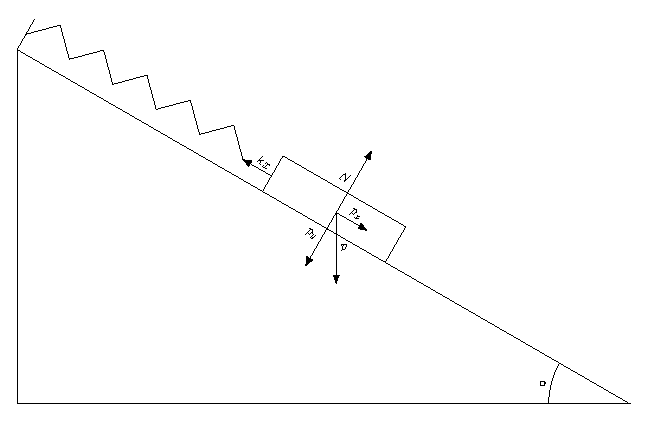
\includegraphics[width=\textwidth]{dibujillo.eps}
\end{minipage}
\begin{minipage}{0.5\textwidth}
\begin{align*}
g &= 10 \, \text{m}/\text{s}^2 \text{\ gravedad/gravity}\\
k &= 60 \, \text{N}/\text{m} \text{\ constante del muelle/ spring constant}\\
m &= 2 \, \text{kg} \text{\ masa del bloque/block mass}\\
\alpha &= \frac{\pi}{6} \text{\ ángulo del plano inclinado/inclined plane angle}\\
N &= \text{Reacción normal del plano/ plane normal force}\\
p &= mg\\
	\mu &= 0.1 \, \text{kg}/\text{s} \text{\ coeficiente de rozamiento/friction coefficient}\\
\end{align*}

\end{minipage}
\bicaption{Sistema masa-muelle-plano inclinado.}{Mass-spring-inclined plane system.}
\label{fig1}
\end{figure}

Sobre un plano inclinado se coloca un bloque sujeto por un muelle, tal y como muestra en la Figura \ref{fig1}. La superficie de contacto entre el bloque y el plano está muy pulida; por lo que se puede considerar que el rozamiento entre ambos es proporcional a la velocidad $v_x(t(t))\in\mathbb{R}$ a lo largo del eje paralelo al plano.

El movimiento del bloque en la dirección del plano puede determinarse mediante la ecuación

\begin{equation}
	ma_{x}(t) = -kx(t) -\mu \lvert N \lvert v_x(t) + p_x, \label{eq: f}
\end{equation}
donde $a(t)\in\mathbb{R}$ representa la aceleración del bloque,$v_x(t) \in\mathbb{R}$ la velocidad, $x(t)\in\mathbb{R}$ su posición y el resto constantes se describen en la Figura \ref{fig1}. El origen, $x=0$, se toma en el punto en donde la fuerza recuperadora del muelle es nula. La posición crece en el sentido de bajada a lo largo del plano.

\paragraph{1.} \label{p1} Emplea el método de Euler para estimar las posición $x(t)$ y la velocidad $v_x(t)$ del bloque a partir de la ecuación (\ref{eq: f}). Utiliza un paso de integración $h =10^{-3}\text{s}$. Considera una posición inicial $x(0) =0\text{m}$, una velocidad inicial $v(0) = 0\text{m/s}$ y un tiempo final de integración $t_{f}=11\text{s}$.

\paragraph{2.} \label{p2} Representa gráficamente los resultados obtenidos: Posición frente a tiempo y velocidad frente a tiempo. Emplea una figura distinta para cada representación. No olvides añadir rótulos a los ejes indicando las variables representadas con sus unidades.

\paragraph{3.} La solución analítica del problema, para velocidad inicial $v(0)=0$ y cualquier posición inicial $x(0)$ toma la siguiente forma,
\begin{equation}\label{eq2}
	x(t) = \frac{p_x}{k}-\left(\frac{p_x}{k}-x(0)\right)\frac{\omega_0}{\omega}e^{-\eta t}\cos\left(\omega t-\phi \right)
\end{equation}
donde,
\begin{equation}
\begin{matrix}
\omega_0 = \sqrt{\frac{k}{m}} & \eta = \frac{\mu N}{2m}\\
\ & \ \\
\omega = \sqrt{\omega_0^2 -\eta^2} &
\phi = \arcsin \left(\frac{\eta}{\omega_0}\right)
\end{matrix} \nonumber
\end{equation}
a) Calcula la posición del bloque mediante la ecuación (\ref{eq2}). Emplea para ello el mismo intervalo y los mismos instantes de tiempo empleados en el apartado \ref{p1}. Representa los resultados sobre el gráfico  para la posición calculada mediante el método de Euler que has obtenido en el apartado \ref{p2}. 

b) Representa en un gráfico de barras los residuos resultantes de comparar la solución analítica con la obtenida por el método de Euler.

c) Calcula el error cuadrático medio cometido al emplear el método de Euler. Considera como exacta la solución analítica (\ref{eq2}).


\paragraph{4.} Los instantes de tiempo para los que la posición del bloque alcanza un máximo o un mínimo local pueden obtenerse a partir de la frecuencia de oscilación $\omega$,
\begin{equation}\label{eq4}
t_{max/min} = \frac{n \pi}{\omega}, n = 1,2,3,\cdots, \infty
\end{equation}
a) Emplea las ecuaciones (\ref{eq4}) y (\ref{eq2}) para obtener los primeros 20 puntos singulares (máximos o mínimos) del movimiento del bloque. Represéntalos sobre el gráfico de la posición, obtenido en el apartado 3.b).

b) Utilizando los datos obtenidos en el apartado 4.a), emplea el método de diferencia de dos puntos centrada para obtener las derivadas de las posiciones en los máximos y mínimos locales con respecto al tiempo. Si hay puntos para los que no es posible aplicar este método, calcula su derivada empleando otra aproximación razonable.
 
c) Representa los resultados obtenidos en el apartado anterior sobre el gráfico de la velocidad obtenido en el ejercicio \ref{p2}. A la vista de los resultados, ¿Cómo valorarías la precisión del método empleado para obtener las derivadas? 

\paragraph{5.} A partir de los resultados obtenidos para la velocidad en el apartado \ref{p1}, calcula la posición del bloque en el instante de tiempo $t=1s$ mediante la siguiente integral
\begin{equation}
x(1) = \int_0^1v_x(t)dt,
\end{equation}

a) Emplea para ello el método del trapecio.

b) Compara el resultado con los valores obtenidos tanto mediante el método de Euler como a partir de la solución analítica.



\section{Course 2020/21 test.}
\begin{figure}[h]
\begin{minipage}{0.5\textwidth} \ 
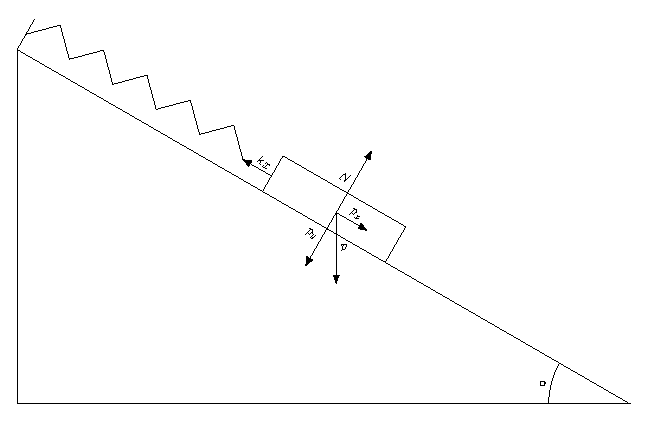
\includegraphics[width=\textwidth]{dibujillo.eps}
\end{minipage}
\begin{minipage}{0.5\textwidth}
\begin{align*}
g &= 10 \, \text{m}/\text{s}^2 \text{\ gravedad/gravity}\\
k &= 60 \, \text{N}/\text{m} \text{\ constante del muelle/ spring constant}\\
m &= 2 \, \text{kg} \text{\ masa del bloque/block mass}\\
\alpha &= \frac{\pi}{6} \text{\ ángulo del plano inclinado/inclined plane angle}\\
N &= \text{Reacción normal del plano/ plane normal force}\\
p &= mg\\
	\mu &= 0.1 \, \text{kg}/\text{s} \text{\ coeficiente de rozamiento/friction coefficient}\\
\end{align*}

\end{minipage}
\bicaption{Sistema masa-muelle-plano inclinado.}{Mass-spring-inclined plane system.}
\label{fig1}
\end{figure}

A block attached to a spring is placed on an inclined plane, as shown in figure \ref{fig1}. The contact surface between the plane and the block is very smooth, and the friction between both then can be considered proportional to the speed $v_x(t(t))\in\mathbb{R}$ along the plane surface.

The displacement of the block along the plane can be described using the following equation,
\begin{equation}
	ma_{x}(t) = -kx(t) -\mu \lvert N \lvert v_x(t) + p_x, \label{eq: f}
\end{equation}

Where  $a(t)\in\mathbb{R}$ represents the block acceleration, $v_x(t) \in\mathbb{R}$ the block velocity, $x(t)\in\mathbb{R}$ its position and the remaining constant are described in figure \ref{fig1}. The coordinate origin $x=0$ is taken where the spring recovery strength is null. The block position increases in the downward direction along the plane.

\paragraph{1.} \label{p1} Employ the Euler's method to stimate the block position $x(t)$ and velocity $v_x(t)$ from equation (\ref{eq: f}). Use a step size $h = 10^{-3}\text{s}$. Take $x(0) = 0\text{m}$ as the initial position, $v(0) = 0\text{m/s}$ as the initial velocity and a final integration time $t_{f}=11\text{s}$.

\paragraph{2.} \label{p2} Represent graphically the results achieved: Position versus time and velocity versus time, using a different figure for each representation. Do not forget to add axis labels indicating the variables and their units.	 

\paragraph{3.} The problem analytical solution, for $v(0)=0$ initial speed and an arbitrary initial position $x(0)$ is, 
\begin{equation}\label{eq2}
	x(t) = \frac{p_x}{k}-\left(\frac{p_x}{k}-x(0)\right)\frac{\omega_0}{\omega}e^{-\eta t}\cos\left(\omega t-\phi \right)
\end{equation}
where,
\begin{equation}
\begin{matrix}
\omega_0 = \sqrt{\frac{k}{m}} & \eta = \frac{\mu N}{2m}\\
\ & \ \\
\omega = \sqrt{\omega_0^2 -\eta^2} &
\phi = \arcsin \left(\frac{\eta}{\omega_0}\right)
\end{matrix} \nonumber
\end{equation}

a) Compute the block position using equation (\ref{eq2}). Employ the same interval and the same time instants, used in section ref{p1}, to do it. Draw the result on top the position graphic computed in section \ref{p2}, using the Euler's method.

b) Compare the analytical solution with Euler's method solution and represent, using a bar graphic, the residual obtained from this comparison.

c) Compute the quadratic error made using the Euler's method. Take the analytical solution as the exact solution.  

\paragraph{4.} We can obtain the time instant at which the block position reaches a local maximum or minimum using the the oscillation frequency $\omega$,
\begin{equation}\label{eq4}
t_{max/min} = \frac{n \pi}{\omega}, n = 1,2,3,\cdots, \infty
\end{equation}

a) Use equations (\ref{eq4}) and (\ref{eq2}) to obtain the first twenty singular points (maxima or minima) for the block displacement. Draw them on top the position graph obtained in section 3.b).  

b) Using the data obtained in section 4.a), employ the two point central difference method to obtain the time derivatives of the block position at the local maxima and minima. It there are points for which it is not possible to apply this method, compute the derivative using another reasonable approach.

c) Represent the result obtained on top of the graphic for the velocity drawn in section \ref{p2}. According to the resulting graphic, how do you consider the precision of the method used for computing the derivatives?

\paragraph{5.} From the results obtained for the velocity in section \ref{p1}, compute the the position of the block at time $t=1s$ using the following integral,  
\begin{equation}
x(1) = \int_0^1v_x(t)dt,
\end{equation}
a) Employ to do it the trapezium formula
b) Compare the results with those obtained from the Euler's method and from the analytical solution.

\section*{LCC. Test 4 (curso 2024 -2025) \protect\footnote{Crea las funciones necesarias  y da los resultados y tus comentarios en un \emph{notebook}.}}

Una de las atracciones de mayor éxito en el parque de atracciones de Gotham es la catapulta de Thalia al Ghul. Los participantes son introducidos en una cápsula esférica transparente y lanzados al aire por la catapulta. La cápsula viaja por el aire hasta alcanzar un lago artificial del parque de atracciones.

Thalia está interesada en saber cual es la mejor ubicación para el lago artificial. Para ello hace uso de sus brillantes conocimientos de física de bachillerato y plantea las siguientes ecuaciones,

\begin{align}
	x &= v_0\cos(\theta)t + x_0 \label{eq1}\\
	h &= -\frac{1}{2}gt^2 + v_0\sin({\theta})t + h_0 \label{eq2}
\end{align}
Donde $v_0$ Representa la velocidad de lanzamiento desde la catapulta en $m/s$, $x_0$ es la posición inicial horizontal de la cápsula en $m$, $h_0$ la altura inicial en $m$, $g=9.8m/s$ la aceleración de la gravedad, $\theta$ el ángulo de lanzamiento en radianes y $t$ el tiempo en segundos.

Lucía y Laura, antiguas compañeras de bachiller de Thalia, se parten de risa al ver sus ecuaciones y le dicen que la cápsula sufre una enorme fuerza de fricción con el aire y que las ecuaciones que plantea no sirven para resolver su problema.

A cambio, le proponen que emplee las siguientes ecuaciones,
\begin{align}
	\frac{dx}{dt} &= v_x \label{eq3}\\
	\frac{dh}{dt} &= v_h\\
	\frac{dv_x}{dt} &= - \frac{C_d}{m}\rho\pi r^2|v|v_x\\
	\frac{dv_h}{dt} &= -g - \frac{C_d}{m}\rho\pi r^2|v|v_h \label{eq5}
\end{align}

Donde $C_d = 0.47$ es el coeficiente de arrastre de una esfera, $\rho = 1.22Kg/m^3$ es la densidad del aire seco a nivel del mar y $30^o$ centígrados de temperatura, $r = 1m$ es el radio de la cápsula esférica y $m=100Kg$ su masa. El resto de variables son iguales a las de las primeras ecuaciones.

Thalia, que no tiene la menor idea de como resolver las ecuaciones que le plantean, enfurece y amenaza a Lucía y a Laura con echarles encima a la Liga de Asesinos si no le resuelven el problema.

Laura y Lucía piden ayuda al resto de sus compañeros de LCC a ver si entre todos consiguen resolverlo.

\begin{enumerate}
	\item (\textbf{2 ptos}) Emplea las ecuaciones (\ref{eq1}) y (\ref{eq2}) para obtener las posiciones sucesivas de la cápsula desde su lanzamiento hasta que toca la superficie del lago. Considera que la velocidad con la que sale la cápsula de la catapulta es $v_0 = 20 m/s$ y sale formando un ángulo $\theta = \pi/3$ con la horizontal. La altura desde la que sale es $h_0 = 2m$. Toma $x_0=0m$. Dibuja la trayectoria. (Aunque sabemos que no es necesario recordároslo el tiempo máximo de vuelo para el tiro parabólico se puede calcular como $t_{max} = \frac{v_{0y} + \sqrt{v_{0y}^2+2gh_0}}{g}$)
	
	
	\item (\textbf{4 ptos}) Emplea el método de Euler para resolver las ecuaciones (\ref{eq3}) - (\ref{eq5}). Toma para las posiciones y velocidades iniciales los mismo valores del apartado anterior. Integra hasta que la cápsula toque o rebase la superficie del lago. Emplea un incremento de tiempo $\Delta t = 0.0001$. Dibuja la trayectoria resultante en el mismo gráfico del ejercicio anterior.
	A la vista de los resultados, indica si era acertada la sugerencia de Lucía y Laura.
	
	\item \textbf{Bonus track}(\textbf{1 pto}) El cálculo realizado solo el válido para días sin viento, ya que la velocidad empleada para calcular la fricción es relativa al aire. Vuelve a resolver el problema suponiendo una velocidad horizontal del viento $v_{xaire} = -10 m/s$. Compara con los resultados anteriores.
\end{enumerate}
Laura y Lucía se han venido arriba y deciden emplear los resultados anteriores para estimar el trabajo realizado por la fricción del aire y comprobar si son ciertos los teoremas de conservación de la energía.
Para ello, parten de la ecuación del trabajo de una fuerza,
\begin{equation}\label{eq7}
	W = \int_0^R F_r\cdot ds = \int_{x_0}^{x_{fin}}F_{rx}dx + \int_{h_0}^{h_{fin}} F_{rh}dh
\end{equation}
Con,
\begin{align}
	F_{rx} = - C_d\rho\pi r^2|v|v_x\\
	F_{rh} = - C_d\rho\pi r^2|v|v_h
\end{align}
\begin{enumerate}[resume]
	\item (\textbf{4 ptos}) Empleando el método del trapecio y los valores de $(x,v_x)$, y $(h,v_h)$ obtenidos en el apartado (2), calcula el trabajo realizado por la fricción del aire a partir del término de la derecha de la ecuación (\ref{eq7}).
	Comprueba que, efectivamente, se aproxima a la pérdida de energía de la cápsula desde su lanzamiento hasta que toca la superficie del agua. (Ten en cuenta que el cálculo es sólo aproximado y mejora si vuelves a obtener la solución mediante el método de Euler, empleando pasos de tiempo más pequeños) \footnote{Si te has atascado en el ejercicio 2 y no tienes los valores de  $(x,v_x)$, y $(h,v_h)$ puedes descargarlos del fichero \textit{"datosLauraLucia.txt"} del campus virtual.}
\end{enumerate}